\documentclass[a4paper]{article}

\def\npart {IB}
\def\nterm {Lent}
\def\nyear {2015}
\def\nlecturer {D.\ Spiegelhalter}
\def\ncourse {Statistics}
\def\nofficial {http://www.statslab.cam.ac.uk/Dept/People/djsteaching/S1B-15-all-lectures.pdf}

% Imports
\ifx \nextra \undefined
  \usepackage[pdftex,
    hidelinks,
    pdfauthor={Dexter Chua},
    pdfsubject={Cambridge Maths Notes: Part \npart\ - \ncourse},
    pdftitle={Part \npart\ - \ncourse},
  pdfkeywords={Cambridge Mathematics Maths Math \npart\ \nterm\ \nyear\ \ncourse}]{hyperref}
  \title{Part \npart\ - \ncourse}
\else
  \usepackage[pdftex,
    hidelinks,
    pdfauthor={Dexter Chua},
    pdfsubject={Cambridge Maths Notes: Part \npart\ - \ncourse\ (\nextra)},
    pdftitle={Part \npart\ - \ncourse\ (\nextra)},
  pdfkeywords={Cambridge Mathematics Maths Math \npart\ \nterm\ \nyear\ \ncourse\ \nextra}]{hyperref}

  \title{Part \npart\ - \ncourse \\ {\Large \nextra}}
\fi

\author{Lectured by \nlecturer \\\small Notes taken by Dexter Chua}
\date{\nterm\ \nyear}

\usepackage{alltt}
\usepackage{amsfonts}
\usepackage{amsmath}
\usepackage{amssymb}
\usepackage{amsthm}
\usepackage{booktabs}
\usepackage{caption}
\usepackage{enumitem}
\usepackage{fancyhdr}
\usepackage{graphicx}
\usepackage{mathtools}
\usepackage{microtype}
\usepackage{multirow}
\usepackage{pdflscape}
\usepackage{pgfplots}
\usepackage{siunitx}
\usepackage{tabularx}
\usepackage{tikz}
\usepackage{tkz-euclide}
\usepackage[normalem]{ulem}
\usepackage[all]{xy}

\pgfplotsset{compat=1.12}

\pagestyle{fancyplain}
\lhead{\emph{\nouppercase{\leftmark}}}
\ifx \nextra \undefined
  \rhead{
    \ifnum\thepage=1
    \else
      \npart\ \ncourse
    \fi}
\else
  \rhead{
    \ifnum\thepage=1
    \else
      \npart\ \ncourse\ (\nextra)
    \fi}
\fi
\usetikzlibrary{arrows}
\usetikzlibrary{decorations.markings}
\usetikzlibrary{decorations.pathmorphing}
\usetikzlibrary{positioning}
\usetikzlibrary{fadings}
\usetikzlibrary{intersections}
\usetikzlibrary{cd}

\newcommand*{\Cdot}{\raisebox{-0.25ex}{\scalebox{1.5}{$\cdot$}}}
\newcommand {\pd}[2][ ]{
  \ifx #1 { }
    \frac{\partial}{\partial #2}
  \else
    \frac{\partial^{#1}}{\partial #2^{#1}}
  \fi
}

% Theorems
\theoremstyle{definition}
\newtheorem*{aim}{Aim}
\newtheorem*{axiom}{Axiom}
\newtheorem*{claim}{Claim}
\newtheorem*{cor}{Corollary}
\newtheorem*{defi}{Definition}
\newtheorem*{eg}{Example}
\newtheorem*{fact}{Fact}
\newtheorem*{law}{Law}
\newtheorem*{lemma}{Lemma}
\newtheorem*{notation}{Notation}
\newtheorem*{prop}{Proposition}
\newtheorem*{thm}{Theorem}

\renewcommand{\labelitemi}{--}
\renewcommand{\labelitemii}{$\circ$}
\renewcommand{\labelenumi}{(\roman{*})}

\let\stdsection\section
\renewcommand\section{\newpage\stdsection}

% Strike through
\def\st{\bgroup \ULdepth=-.55ex \ULset}

% Maths symbols
\newcommand{\bra}{\langle}
\newcommand{\ket}{\rangle}

\newcommand{\N}{\mathbb{N}}
\newcommand{\Z}{\mathbb{Z}}
\newcommand{\Q}{\mathbb{Q}}
\renewcommand{\H}{\mathbb{H}}
\newcommand{\R}{\mathbb{R}}
\newcommand{\C}{\mathbb{C}}
\newcommand{\Prob}{\mathbb{P}}
\renewcommand{\P}{\mathbb{P}}
\newcommand{\E}{\mathbb{E}}
\newcommand{\F}{\mathbb{F}}
\newcommand{\cU}{\mathcal{U}}
\newcommand{\RP}{\mathbb{RP}}
\newcommand{\CP}{\mathbb{CP}}

\newcommand{\ph}{\,\cdot\,}

\DeclareMathOperator{\sech}{sech}
\DeclareMathOperator{\cosech}{cosech}
\DeclareMathOperator{\cosec}{cosec}

\DeclareMathOperator{\covol}{covol}
\DeclareMathOperator{\vol}{vol}

\let\Im\relax
\let\Re\relax
\DeclareMathOperator{\Im}{Im}
\DeclareMathOperator{\Re}{Re}
\DeclareMathOperator{\im}{im}
\DeclareMathOperator{\image}{image}
\DeclareMathOperator{\Ann}{Ann}

\DeclareMathOperator*{\res}{res}
\DeclareMathOperator{\Res}{Res}
\DeclareMathOperator{\Ind}{Ind}

\DeclareMathOperator{\tr}{tr}
\DeclareMathOperator{\diag}{diag}
\DeclareMathOperator{\rank}{rank}
\DeclareMathOperator{\card}{card}
\DeclareMathOperator{\spn}{span}
\DeclareMathOperator{\adj}{adj}

\DeclareMathOperator{\erf}{erf}
\DeclareMathOperator{\erfc}{erfc}

\DeclareMathOperator{\ord}{ord}
\DeclareMathOperator{\Sym}{Sym}

\DeclareMathOperator{\sgn}{sgn}
\DeclareMathOperator{\orb}{orb}
\DeclareMathOperator{\stab}{stab}
\DeclareMathOperator{\ccl}{ccl}

\DeclareMathOperator{\lcm}{lcm}
\DeclareMathOperator{\hcf}{hcf}

\DeclareMathOperator{\Int}{Int}
\DeclareMathOperator{\id}{id}

\DeclareMathOperator{\betaD}{beta}
\DeclareMathOperator{\gammaD}{gamma}
\DeclareMathOperator{\Poisson}{Poisson}
\DeclareMathOperator{\binomial}{binomial}
\DeclareMathOperator{\multinomial}{multinomial}
\DeclareMathOperator{\Bernoulli}{Bernoulli}
\DeclareMathOperator{\like}{like}

\DeclareMathOperator{\var}{var}
\DeclareMathOperator{\cov}{cov}
\DeclareMathOperator{\bias}{bias}
\DeclareMathOperator{\mse}{mse}
\DeclareMathOperator{\corr}{corr}

\DeclareMathOperator{\otp}{otp}
\DeclareMathOperator{\dom}{dom}

\DeclareMathOperator{\Root}{Root}
\DeclareMathOperator{\supp}{supp}
\DeclareMathOperator{\rel}{rel}
\DeclareMathOperator{\Hom}{Hom}
\DeclareMathOperator{\Aut}{Aut}
\DeclareMathOperator{\Gal}{Gal}
\DeclareMathOperator{\Mat}{Mat}
\DeclareMathOperator{\End}{End}
\DeclareMathOperator{\Char}{char}
\DeclareMathOperator{\ev}{ev}
\DeclareMathOperator{\St}{St}
\DeclareMathOperator{\Lk}{Lk}
\DeclareMathOperator{\disc}{disc}
\DeclareMathOperator{\Isom}{Isom}
\DeclareMathOperator{\length}{length}
\DeclareMathOperator{\energy}{energy}
\DeclareMathOperator{\area}{area}
\DeclareMathOperator{\Syl}{Syl}
\DeclareMathOperator{\cl}{cl}
\DeclareMathOperator{\fix}{fix}

\newcommand{\GL}{\mathrm{GL}}
\newcommand{\SL}{\mathrm{SL}}
\newcommand{\PGL}{\mathrm{PGL}}
\newcommand{\PSL}{\mathrm{PSL}}
\newcommand{\PSU}{\mathrm{PSU}}
\newcommand{\Or}{\mathrm{O}}
\newcommand{\SO}{\mathrm{SO}}
\newcommand{\U}{\mathrm{U}}
\newcommand{\SU}{\mathrm{SU}}

\renewcommand{\d}{\mathrm{d}}
\newcommand{\D}{\mathrm{D}}

\tikzset{->/.style = {decoration={markings,
                                  mark=at position 1 with {\arrow[scale=2]{latex'}}},
                      postaction={decorate}}}
\tikzset{<-/.style = {decoration={markings,
                                  mark=at position 0 with {\arrowreversed[scale=2]{latex'}}},
                      postaction={decorate}}}
\tikzset{<->/.style = {decoration={markings,
                                   mark=at position 0 with {\arrowreversed[scale=2]{latex'}},
                                   mark=at position 1 with {\arrow[scale=2]{latex'}}},
                       postaction={decorate}}}
\tikzset{->-/.style = {decoration={markings,
                                   mark=at position #1 with {\arrow[scale=2]{latex'}}},
                       postaction={decorate}}}
\tikzset{-<-/.style = {decoration={markings,
                                   mark=at position #1 with {\arrowreversed[scale=2]{latex'}}},
                       postaction={decorate}}}

\tikzset{circ/.style = {fill, circle, inner sep = 0, minimum size = 3}}
\tikzset{mstate/.style={circle, draw, blue, text=black, minimum width=0.7cm}}

\definecolor{mblue}{rgb}{0.2, 0.3, 0.8}
\definecolor{morange}{rgb}{1, 0.5, 0}
\definecolor{mgreen}{rgb}{0.1, 0.4, 0.2}
\definecolor{mred}{rgb}{0.5, 0, 0}

\def\drawcirculararc(#1,#2)(#3,#4)(#5,#6){%
    \pgfmathsetmacro\cA{(#1*#1+#2*#2-#3*#3-#4*#4)/2}%
    \pgfmathsetmacro\cB{(#1*#1+#2*#2-#5*#5-#6*#6)/2}%
    \pgfmathsetmacro\cy{(\cB*(#1-#3)-\cA*(#1-#5))/%
                        ((#2-#6)*(#1-#3)-(#2-#4)*(#1-#5))}%
    \pgfmathsetmacro\cx{(\cA-\cy*(#2-#4))/(#1-#3)}%
    \pgfmathsetmacro\cr{sqrt((#1-\cx)*(#1-\cx)+(#2-\cy)*(#2-\cy))}%
    \pgfmathsetmacro\cA{atan2(#2-\cy,#1-\cx)}%
    \pgfmathsetmacro\cB{atan2(#6-\cy,#5-\cx)}%
    \pgfmathparse{\cB<\cA}%
    \ifnum\pgfmathresult=1
        \pgfmathsetmacro\cB{\cB+360}%
    \fi
    \draw (#1,#2) arc (\cA:\cB:\cr);%
}
\newcommand\getCoord[3]{\newdimen{#1}\newdimen{#2}\pgfextractx{#1}{\pgfpointanchor{#3}{center}}\pgfextracty{#2}{\pgfpointanchor{#3}{center}}}

\def\Xint#1{\mathchoice
   {\XXint\displaystyle\textstyle{#1}}%
   {\XXint\textstyle\scriptstyle{#1}}%
   {\XXint\scriptstyle\scriptscriptstyle{#1}}%
   {\XXint\scriptscriptstyle\scriptscriptstyle{#1}}%
   \!\int}
\def\XXint#1#2#3{{\setbox0=\hbox{$#1{#2#3}{\int}$}
     \vcenter{\hbox{$#2#3$}}\kern-.5\wd0}}
\def\ddashint{\Xint=}
\def\dashint{\Xint-}


\begin{document}
\maketitle
{\small
\noindent\textbf{Estimation}\\
Review of distribution and density functions, parametric families. Examples: binomial, Poisson, gamma. Sufficiency, minimal sufficiency, the Rao-Blackwell theorem. Maximum likelihood estimation. Confidence intervals. Use of prior distributions and Bayesian inference.\hspace*{\fill} [5]

\vspace{10pt}
\noindent\textbf{Hypothesis testing}\\
Simple examples of hypothesis testing, null and alternative hypothesis, critical region, size, power, type I and type II errors, Neyman-Pearson lemma. Significance level of outcome. Uniformly most powerful tests. Likelihood ratio, and use of generalised likelihood ratio to construct test statistics for composite hypotheses. Examples, including $t$-tests and $F$-tests. Relationship with confidence intervals. Goodness-of-fit tests and contingency tables.\hspace*{\fill} [4]

\vspace{10pt}
\noindent\textbf{Linear models}\\
Derivation and joint distribution of maximum likelihood estimators, least squares, Gauss-Markov theorem. Testing hypotheses, geometric interpretation. Examples, including simple linear regression and one-way analysis of variance. Use of software.\hspace*{\fill} [7]}

\tableofcontents

\setcounter{section}{-1}
\section{Introduction}
Statistics is a set of principles and procedures for gaining and processing quantitative evidence in order to help us make judgements and decisions. In this course, we focus on formal \emph{statistical inference}. In the process, we assume that we have some data generated from some unknown probability model, and we aim to use the data to learn about certain properties of the underlying probability model.

In particular, we perform \emph{parametric inference}. We assume that we have a random variable $X$ that follows a particular known family of distribution (e.g.\ Poisson distribution). However, we do not know the parameters of the distribution. We then attempt to estimate the parameter from the data given.

For example, we might know that $X\sim \Poisson (\mu)$ for some $\mu$, and we want to figure out what $\mu$ is.

Usually we repeat the experiment (or observation) many times. Hence we will have $X_1, X_2, \cdots, X_n$ being iid with the same distribution as $X$. We call the set $\mathbf{X} = (X_1, X_2, \cdots, X_n)$ a \emph{simple random sample}. This is the data we have.

We will use the observed $\mathbf{X} = \mathbf{x}$ to make inferences about the parameter $\theta$, such as
\begin{itemize}
  \item giving an estimate $\hat{\theta}(\mathbf{x})$ of the true value of $\theta$.
  \item Giving an interval estimate $(\hat{\theta}_1(\mathbf{x}), \hat{\theta}_2(\mathbf{x}))$ for $\theta$
  \item testing a hypothesis about $\theta$, e.g.\ whether $\theta = 0$.
\end{itemize}
\section{Estimation}
\subsection{Estimators}
The goal of estimation is as follows: we are given iid $X_1, \cdots, X_n$, and we know that their probability density/mass function is $f_X(x; \theta)$ for some unknown $\theta$. We know $f_X$ but not $\theta$. For example, we might know that they follow a Poisson distribution, but we do not know what the mean is. The objective is to estimate the value of $\theta$.

\begin{defi}[Statistic]
  A \emph{statistic} is an estimate of $\theta$. It is a function $T$ of the data. If we write the data as $\mathbf{x} = (x_1, \cdots, x_n)$, then our estimate is written as $\hat{\theta} = T(\mathbf{x})$. $T(\mathbf{X})$ is an \emph{estimator} of $\theta$.

  The distribution of $T = T(\mathbf{X})$ is the \emph{sampling distribution} of the statistic.
\end{defi}
Note that we adopt the convention where capital $\mathbf{X}$ denotes a random variable and $\mathbf{x}$ is an observed value. So $T(\mathbf{X})$ is a random variable and $T(\mathbf{x})$ is a particular value we obtain after experiments.

\begin{eg}
  Let $X_1, \cdots, X_n$ be iid $N(\mu, 1)$. A possible estimator for $\mu$ is
  \[
    T(\mathbf{X}) = \frac{1}{n}\sum X_i.
  \]
  Then for any particular observed sample $\mathbf{x}$, our estimate is
  \[
    T(\mathbf{x}) = \frac{1}{n}\sum x_i.
  \]
  What is the sampling distribution of $T$? Recall from IA Probability that in general, if $X_i \sim N(\mu_i, \sigma_i^2)$, then $\sum X_i \sim N(\sum \mu_i, \sum \sigma_i^2)$, which is something we can prove by considering moment-generating functions.

  So we have $T(\mathbf{X})\sim N(\mu, 1/n)$. Note that by the Central Limit Theorem, even if $X_i$ were not normal, we still have approximately $T(\mathbf{X})\sim N(\mu, 1/n)$ for large values of $n$, but here we get exactly the normal distribution even for small values of $n$.
\end{eg}
The estimator $\frac{1}{n}\sum X_i$ we had above is a rather sensible estimator. Of course, we can also have silly estimators such as $T(\mathbf{X}) = X_1$, or even $T(\mathbf{X}) = 0.32$ always.

One way to decide if an estimator is silly is to look at its \emph{bias}.
\begin{defi}[Bias]
  Let $\hat{\theta} = T(\mathbf{X})$ be an estimator of $\theta$. The \emph{bias} of $\hat{\theta}$ is the difference between its expected value and true value.
  \[
    \bias(\hat{\theta}) = \E_\theta(\hat{\theta}) - \theta.
  \]
  Note that the subscript $_\theta$ does not represent the random variable, but the thing we want to estimate. This is inconsistent with the use for, say, the probability mass function.

  An estimator is \emph{unbiased} if it has no bias, i.e.\ $\E_\theta(\hat{\theta}) = \theta$.
\end{defi}
To find out $\E_\theta (T)$, we can either find the distribution of $T$ and find its expected value, or evaluate $T$ as a function of $\mathbf{X}$ directly, and find its expected value.

\begin{eg}
  In the above example, $\E_\mu(T) =\mu$. So $T$ is unbiased for $\mu$.
\end{eg}

\subsection{Mean squared error}
Given an estimator, we want to know how good the estimator is. We have just come up with the concept of the \emph{bias} above. However, this is generally not a good measure of how good the estimator is.

For example, if we do 1000 random trials $X_1, \cdots, X_{1000}$, we can pick our estimator as $T(\mathbf{X}) = X_1$. This is an unbiased estimator, but is really bad because we have just wasted the data from the other 999 trials. On the other hand, $T'(\mathbf{X}) = 0.01 + \frac{1}{1000}\sum X_i$ is biased (with a bias of $0.01$), but is in general much more trustworthy than $T$. In fact, at the end of the section, we will construct cases where the only possible unbiased estimator is a completely silly estimator to use.

Instead, a commonly used measure is the \emph{mean squared error}.
\begin{defi}[Mean squared error]
  The \emph{mean squared error} of an estimator $\hat{\theta}$ is $\E_\theta[(\hat{\theta} - \theta)^2]$.

  Sometimes, we use the \emph{root mean squared error}, that is the square root of the above.
\end{defi}
We can express the mean squared error in terms of the variance and bias:
\begin{align*}
  \E_\theta[(\hat{\theta} - \theta)^2] &= \E_\theta[(\hat{\theta} - \E_\theta(\hat{\theta}) + \E_\theta(\hat{\theta}) - \theta)^2]\\
  &= \E_\theta[(\hat{\theta} - \E_\theta(\hat{\theta}))^2] + [\E_\theta(\hat{\theta}) - \theta]^2 + 2\E_{\theta}[\E_\theta(\hat{\theta}) - \theta]\underbrace{\E_\theta[\hat{\theta} - \E_\theta(\hat{\theta})]}_{0}\\
  &= \var(\hat{\theta}) + \bias^2(\hat{\theta}).
\end{align*}
If we are aiming for a low mean squared error, sometimes it could be preferable to have a biased estimator with a lower variance. This is known as the ``bias-variance trade-off''.

For example, suppose $X\sim \binomial(n, \theta)$. The standard estimator is $T_U = X/n$, which is unbiased. $T_U$ has variance
\[
  \var_\theta(T_U) = \frac{\var_\theta(X)}{n^2} = \frac{\theta(1 - \theta)}{n}.
\]
Hence the mean squared error of the usual estimator is given by
\[
  \mse (T_U) = \var_\theta(T_U) + \bias^2(T_U) = \theta(1 - \theta)/n.
\]
Consider an alternative estimator
\[
  T_B = \frac{X + 1}{n + 2} = w\frac{X}{n} + (1 - w)\frac{1}{2},
\]
where $w = n/(n + 2)$. This can be interpreted to be a weighted average (by the sample size) of the sample mean and $1/2$. We have
\[
  \E_\theta(T_B) - \theta = \frac{n\theta + 1}{n + 2} - \theta = (1 - w)\left(\frac{1}{2} - \theta\right),
\]
and is biased. The variance is given by
\[
  \var_\theta(T_B) = \frac{\var_\theta(X)}{(n + 2)^2} = w^2\frac{\theta(1 - \theta)}{n}.
\]
Hence the mean squared error is
\[
  \mse (T_B) = \var_\theta(T_B) + \bias^2(T_B) = w^2\frac{\theta(1 - \theta)}{n} + (1 - w)^2\left(\frac{1}{2} - \theta\right)^2.
\]
We can plot the mean squared error of each estimator for possible values of $\theta$. Here we plot the case where $n = 10$.
\begin{center}
  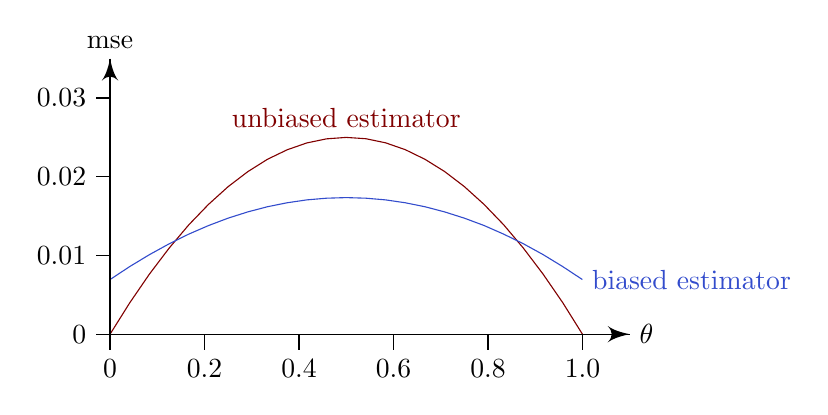
\begin{tikzpicture}[xscale=6,yscale=100]
    \draw [mred, domain=0:1] plot (\x, {\x * (1 - \x) / 10});
    \node [mred, above] at (0.5, 0.025) {unbiased estimator};
    \draw [mblue, domain=0:1] plot (\x, {25 * \x * (1 - \x) / 360 + (1 - 5/6)*(1 - 5/6)*(0.5 - \x)*(0.5 - \x)}) node [right] {biased estimator};
    \draw [->] (0, 0) -- (1.1, 0) node [right] {$\theta$};
    \draw [->] (0, 0) -- (0, 0.035) node [above] {mse};
    \foreach \x in {0, 0.2, 0.4, 0.6, 0.8, 1.0} {
      \draw (\x, 0) -- (\x, -0.002) node [below] {\x};
    }
    \foreach \y in {0, 0.01, 0.02, 0.03} {
      \draw (0, \y) -- (-.03, \y) node [left] {\y};
    }
  \end{tikzpicture}
\end{center}
This biased estimator has smaller MSE unless $\theta$ has extreme values.

We see that sometimes biased estimators could give better mean squared errors. In some cases, not only could unbiased estimators be worse --- they could be completely nonsense.

Suppose $X\sim \Poisson(\lambda)$, and for some reason, we want to estimate $\theta = [P(X = 0)]^2 = e^{-2\lambda}$. Then any unbiased estimator $T(X)$ must satisfy $\E_\theta(T(X)) = \theta$, or equivalently,
\[
  E_\lambda(T(X)) = e^{-\lambda}\sum_{x = 0}^\infty T(x) \frac{\lambda^x}{x!} = e^{-2\lambda}.
\]
The only function $T$ that can satisfy this equation is $T(X) = (-1)^X$.

Thus the unbiased estimator would estimate $e^{-2\lambda}$ to be $1$ if $X$ is even, -1 if $X$ is odd. This is clearly nonsense.
\subsection{Sufficiency}
Often, we do experiments just to find out the value of $\theta$. For example, we might want to estimate what proportion of the population supports some political candidate. We are seldom interested in the data points themselves, and just want to learn about the big picture. This leads us to the concept of a \emph{sufficient statistic}. This is a statistic $T(\mathbf{X})$ that contains all information we have about $\theta$ in the sample.

\begin{eg}
  Let $X_1, \cdots X_n$ be iid $\Bernoulli(\theta)$, so that $\P(X_i = 1) = 1 - \P(X_i = 0) = \theta$ for some $0 < \theta < 1$. So
  \[
    f_{\mathbf{X}} (\mathbf{x}\mid \theta) = \prod_{i = 1}^n \theta^{x_i}(1 - \theta)^{1 - x_i} = \theta^{\sum x_i}(1 - \theta)^{n - \sum x_i}.
  \]
  This depends on the data only through $T(\mathbf{X}) = \sum x_i$, the total number of ones.

  Suppose we are now given that $T(\mathbf{X}) = t$. Then what is the distribution of $\mathbf{X}$? We have
  \[
    f_{\mathbf{X}\mid T = t}(\mathbf{x}) = \frac{\P_\theta(\mathbf{X} = \mathbf{x}, T = t)}{\P_\theta (T = t)} = \frac{\P_\theta(\mathbf{X} = \mathbf{x})}{\P_\theta(T = t)}.
  \]
  Where the last equality comes because since if $\mathbf{X} = \mathbf{x}$, then $T$ must be equal to $t$. This is equal to
  \[
    \frac{\theta^{\sum x_i}(1 - \theta)^{n - \sum x_i}}{\binom{n}{t}\theta^t (1 - \theta)^{n - t}} = \binom{n}{t}^{-1}.
  \]
  So the conditional distribution of $\mathbf{X}$ given $T = t$ does not depend on $\theta$. So if we know $T$, then additional knowledge of $\mathbf{x}$ does not give more information about $\theta$.
\end{eg}

\begin{defi}[Sufficient statistic]
  A statistic $T$ is \emph{sufficient} for $\theta$ if the conditional distribution of $\mathbf{X}$ given $T$ does not depend on $\theta$.
\end{defi}

There is a convenient theorem that allows us to find sufficient statistics.
\begin{thm}[The factorization criterion]
  $T$ is sufficient for $\theta$ if and only if
  \[
    f_{\mathbf{X}}(\mathbf{x} \mid \theta) = g(T(\mathbf{x}), \theta)h(\mathbf{x})
  \]
  for some functions $g$ and $h$.
\end{thm}

\begin{proof}
  We first prove the discrete case.

  Suppose $f_\mathbf{X}(\mathbf{x}\mid \theta) = g(T(\mathbf{x}), \theta)h(\mathbf{x})$. If $T(\mathbf{x}) = t$, then
  \begin{align*}
    f_{\mathbf{X}\mid T = t}(\mathbf{x}) &= \frac{\P_\theta(\mathbf{X} = \mathbf{x}, T(\mathbf{X}) = t)}{\P_\theta (T = t)}\\
    &= \frac{g(T(\mathbf{x}), \theta)h(\mathbf{x})}{\sum_{\{\mathbf{y}:T(\mathbf{y}) = t\}}g(T(\mathbf{y}), \theta)h(\mathbf{y})}\\
    &=\frac{g(t, \theta)h(\mathbf{x})}{g(t, \theta)\sum h(\mathbf{y})}\\
    &= \frac{h(\mathbf{x})}{\sum h(\mathbf{y})}
  \end{align*}
  which doesn't depend on $\theta$. So $T$ is sufficient.

  The continuous case is similar. If $f_\mathbf{X}(\mathbf{x} \mid \theta) = g(T(\mathbf{x}), \theta)h(\mathbf{x})$, and $T(\mathbf{x}) = t$, then
  \begin{align*}
    f_{\mathbf{X}\mid T = t}(\mathbf{x}) &= \frac{g(T(\mathbf{x}), \theta) h(\mathbf{x})}{\int_{\mathbf{y}: T(\mathbf{y}) = t} g(T(\mathbf{y}), \theta) h(\mathbf{y})\;\d \mathbf{y}}\\
    &= \frac{g(t, \theta) h(\mathbf{x})}{g(t, \theta) \int h(\mathbf{y}) \;\d \mathbf{y}}\\
    &= \frac{h(\mathbf{x})}{\int h(\mathbf{y})\;\d \mathbf{y}},
  \end{align*}
  which does not depend on $\theta$.

  Now suppose $T$ is sufficient so that the conditional distribution of $\mathbf{X}\mid T = t$ does not depend on $\theta$. Then
  \[
    \P_\theta(\mathbf{X} = \mathbf{x}) = \P_\theta(\mathbf{X} = \mathbf{x}, T=T(\mathbf{x})) = \P_\theta(\mathbf{X} = \mathbf{x}\mid T = T(\mathbf{x}))\P_\theta (T = T(\mathbf{x})).
  \]
  The first factor does not depend on $\theta$ by assumption; call it $h(\mathbf{x})$. Let the second factor be $g(t, \theta)$, and so we have the required factorisation.
\end{proof}

\begin{eg}
  Continuing the above example,
  \[
    f_\mathbf{X}(\mathbf{x}\mid \theta) = \theta^{\sum x_i}(1 - \theta)^{n - \sum x_i}.
  \]
  Take $g(t, \theta) = \theta^t(1 - \theta)^{n - t}$ and $h(\mathbf{x}) = 1$ to see that $T(\mathbf{X}) = \sum X_i$ is sufficient for $\theta$.
\end{eg}

\begin{eg}
  Let $X_1, \cdots, X_n$ be iid $U[0, \theta]$. Write $1_{[A]}$ for the indicator function of an arbitrary set $A$. We have
  \[
    f_\mathbf{X}(\mathbf{x}\mid \theta) = \prod_{i = 1}^n \frac{1}{\theta}1_{[0 \leq x_i\leq \theta]} = \frac{1}{\theta^n}1_{[\max_i x_i \leq \theta]}1_{[\min_i x_i\geq 0]}.
  \]
  If we let $T = \max_i x_i$, then we have
  \[
    f_\mathbf{X}(\mathbf{x}\mid \theta) = \underbrace{\frac{1}{\theta^n}1_{[t \leq \theta]}}_{g(t, \theta)}\quad \underbrace{1_{[\min_i x_i \geq 0]}}_{h(\mathbf{x})}.
  \]
  So $T = \max_i x_i$ is sufficient.
\end{eg}

Note that sufficient statistics are not unique. If $T$ is sufficient for $\theta$, then so is any 1-1 function of $T$. $\mathbf{X}$ is always sufficient for $\theta$ as well, but it is not of much use. How can we decide if a sufficient statistic is ``good''?

Given any statistic $T$, we can partition the sample space $\mathcal{X}^n$ into sets $\{\mathbf{x}\in \mathcal{X}: T(\mathbf{x}) = t\}$. Then after an experiment, instead of recording the actual value of $\mathbf{x}$, we can simply record the partition $\mathbf{x}$ falls into. If there are less partitions than possible values of $\mathbf{x}$, then effectively there is less information we have to store.

If $T$ is sufficient, then this data reduction does not lose any information about $\theta$. The ``best'' sufficient statistic would be one in which we achieve the maximum possible reduction. This is known as the \emph{minimal sufficient statistic}. The formal definition we take is the following:

\begin{defi}[Minimal sufficiency]
  A sufficient statistic $T(\mathbf{X})$ is \emph{minimal} if it is a function of every other sufficient statistic, i.e.\ if $T'(\mathbf{X})$ is also sufficient, then $T'(\mathbf{X}) = T'(\mathbf{Y}) \Rightarrow T(\mathbf{X}) = T(\mathbf{Y})$.
\end{defi}

Again, we have a handy theorem to find minimal statistics:
\begin{thm}
  Suppose $T = T(\mathbf{X})$ is a statistic that satisfies
  \begin{center}
    $\displaystyle\frac{f_\mathbf{X}(\mathbf{x}; \theta)}{f_\mathbf{X}(\mathbf{y}; \theta)}$ does not depend on $\theta$ if and only if $T(\mathbf{x}) = T(\mathbf{y})$.
  \end{center}
  Then $T$ is minimal sufficient for $\theta$.
\end{thm}
\begin{proof}
  First we have to show sufficiency. We will use the factorization criterion to do so.

  Firstly, for each possible $t$, pick a favorite $\mathbf{x}_t$ such that $T(\mathbf{x}_t) = t$.

  Now let $\mathbf{x}\in \mathcal{X}^N$ and let $T(\mathbf{x}) = t$. So $T(\mathbf{x}) = T(\mathbf{x}_t)$. By the hypothesis, $\frac{f_\mathbf{X}(\mathbf{x}; \theta)}{f_\mathbf{X}(\mathbf{x}_t: \theta)}$ does not depend on $\theta$. Let this be $h(\mathbf{x})$. Let $g(t, \theta) = f_\mathbf{X}(\mathbf{x}_t, \theta)$. Then
  \[
    f_\mathbf{X}(\mathbf{x}; \theta) = f_\mathbf{X}(\mathbf{x}_t; \theta) \frac{f_\mathbf{X}(\mathbf{x}; \theta)}{f_\mathbf{X}(\mathbf{x}_t; \theta)} = g(t, \theta) h(\mathbf{x}).
  \]
  So $T$ is sufficient for $\theta$.

  To show that this is minimal, suppose that $S(\mathbf{X})$ is also sufficient. By the factorization criterion, there exist functions $g_S$ and $h_S$ such that
  \[
    f_\mathbf{X}(\mathbf{x}; \theta) = g_S(S(\mathbf{x}), \theta) h_S(\mathbf{x}).
  \]
  Now suppose that $S(\mathbf{x}) = S(\mathbf{y})$. Then
  \[
    \frac{f_\mathbf{X}(\mathbf{x}; \theta)}{f_\mathbf{X}(\mathbf{y}; \theta)} = \frac{g_S(S(\mathbf{x}), \theta)h_S(\mathbf{x})}{g_S(S(\mathbf{y}), \theta)h_S(\mathbf{y})} = \frac{h_S(\mathbf{x})}{h_S(\mathbf{y})}.
  \]
  This means that the ratio $\frac{f_\mathbf{X}(\mathbf{x}; \theta)}{f_\mathbf{X}(\mathbf{y}; \theta)}$ does not depend on $\theta$. By the hypothesis, this implies that $T(\mathbf{x}) = T(\mathbf{y})$. So we know that $S(\mathbf{x}) = S(\mathbf{y})$ implies $T(\mathbf{x}) = T(\mathbf{y})$. So $T$ is a function of $S$. So $T$ is minimal sufficient.
\end{proof}

\begin{eg}
  Suppose $X_1, \cdots, X_n$ are iid $N(\mu, \sigma^2)$. Then
  \begin{align*}
    \frac{f_\mathbf{X}(\mathbf{x}\mid \mu, \sigma^2)}{f_\mathbf{X}(\mathbf{y}\mid \mu, \sigma^2)} &= \frac{(2\pi\sigma^2)^{-n/2}\exp\left\{-\frac{1}{2\sigma^2}\sum_i(x_i - \mu)^2\right\}}{(2\pi\sigma^2)^{-n/2}\exp\left\{-\frac{1}{2\sigma^2}\sum_i(y_i - \mu)^2\right\}}\\
    &=\exp\left\{-\frac{1}{2\sigma^2}\left(\sum_i x_i^2 - \sum_i y_i^2\right) + \frac{\mu}{\sigma^2}\left(\sum_{i}x_i - \sum_i y_i\right)\right\}.
  \end{align*}
  This is a constant function of $(\mu, \sigma^2)$ iff $\sum_i x_i^2 = \sum_i y_i^2$ and $\sum_i x_i = \sum_i y_i$. So $T(\mathbf{X}) = (\sum_i X_i^2, \sum_i X_i)$ is minimal sufficient for $(\mu, \sigma^2)$.
\end{eg}

As mentioned, minimal sufficient statistics allow us to store the results of our experiments in the most efficient way. It turns out if we have a minimal sufficient statistic, then we can use it to improve \emph{any} estimator.
\begin{thm}[Rao-Blackwell Theorem]
  Let $T$ be a sufficient statistic for $\theta$ and let $\tilde{\theta}$ be an estimator for $\theta$ with $\E(\tilde{\theta}^2) < \infty$ for all $\theta$. Let $\hat{\theta}(\mathbf{x}) = \E[\tilde{\theta}(\mathbf{X})\mid T(\mathbf{X}) = T(\mathbf{x})]$. Then for all $\theta$,
  \[
    \E[(\hat{\theta} - \theta)^2] \leq \E[(\tilde{\theta} - \theta)^2].
  \]
  The inequality is strict unless $\tilde{\theta}$ is a function of $T$.
\end{thm}
Here we have to be careful with our definition of $\hat{\theta}$. It is defined as the expected value of $\tilde{\theta}(\mathbf{X})$. And this could potentially depend on the actual value of $\theta$. Fortunately, since $T$ is sufficient for $\theta$, the conditional distribution of $\mathbf{X}$ given $T = t$ does not depend on $\theta$. Hence $\hat{\theta} = \E[\tilde{\theta}(\mathbf{X})\mid T]$ does not depend on $\theta$, and so is a genuine estimator.

Using this theorem, given any estimator, we can find one that is a function of a sufficient statistic and is at least as good in terms of mean squared error of estimation. Moreover, if the original estimator $\tilde{\theta}$ is unbiased, so is the new $\hat{\theta}$. Also, if $\tilde{\theta}$ is already a function of $T$, then $\hat{\theta} = \tilde{\theta}$.

\begin{proof}
  By the conditional expectation formula, we have $\E(\hat{\theta}) = \E[\E(\tilde{\theta}\mid T)] = E(\tilde{\theta})$. So they have the same bias.

  By the conditional variance formula,
  \[
    \var(\tilde{\theta}) = \E[\var (\tilde{\theta}\mid T)] + \var [\E(\tilde{\theta}\mid T)] = \E[\var(\tilde{\theta}\mid T)] + \var(\hat{\theta}).
  \]
  Hence $\var(\tilde{\theta}) \geq \var (\hat{\theta})$. So $\mse(\tilde{\theta}) \geq \mse(\hat{\theta})$, with equality only if $\var(\tilde{\theta}\mid T) = 0$.
\end{proof}

\begin{eg}
  Suppose $X_1, \cdots, X_n$ are iid $\Poisson(\lambda)$, and let $\theta = e^{-\lambda}$, which is the probability that $X_1 = 0$. Then
  \[
    p_\mathbf{X}(\mathbf{x}\mid \lambda) =\frac{-e^{n\lambda}\lambda^{\sum x_i}}{\prod x_i!}.
  \]
  So
  \[
    p_\mathbf{X}(\mathbf{x}\mid \theta) = \frac{\theta^n(-\log \theta)^{\sum x_i}}{\prod x_i!}.
  \]
  We see that $T = \sum X_i$ is sufficient for $\theta$, and $\sum X_i \sim \Poisson (n\lambda)$.

  We start with an easy estimator $\theta$ is $\tilde{\theta} = 1_{X_1 = 0}$, which is unbiased (i.e.\ if we observe nothing in the first observation period, we assume the event is impossible). Then
  \begin{align*}
    \E[\tilde{\theta}\mid T = t] &= \P\left(X_1 = 0 \mid \sum_1^n X_i = t\right)\\
    &= \frac{\P(X_1 = 0)\P(\sum_2^n X_i = t)}{\P(\sum_1^n X_i = t)}\\
    &= \left(\frac{n - 1}{n}\right)^t.
  \end{align*}
  So $\hat{\theta} = (1 - 1/n)^{\sum x_i}$. This approximately $(1 - 1/n)^{n\bar{X}} \approx e^{-\bar X} = e^{-\hat{\lambda}}$, which makes sense.
\end{eg}

\begin{eg}
  Let $X_1, \cdots, X_n$ be iid $U[0, \theta]$, and suppose that we want to estimate $\theta$. We have shown above that $T = \max X_i$ is sufficient for $\theta$. Let $\hat{\theta} = 2X_1$, an unbiased estimator. Then
  \begin{align*}
    \E[\tilde{\theta}\mid T = t] &= 2\E[X_1\mid \max X_i = t]\\
    &= 2\E[X_1\mid \max X_i = t, X_1 = \max X_i]\P(X_1 = \max X_i)\\
    &\quad\quad+ 2\E[X_1\mid \max X_i = t, X_1 \not= \max X_i] \P(X_1 \not= \max X_i)\\
    &= 2\left(t\times \frac{1}{n} + \frac{t}{2}\frac{n - 1}{n}\right)\\
    &= \frac{n + 1}{n}t.
  \end{align*}
  So $\hat{\theta} = \frac{n + 1}{n}\max X_i$ is our new estimator.
\end{eg}

\subsection{Likelihood}
There are many different estimators we can pick, and we have just come up with some criteria to determine whether an estimator is ``good''. However, these do not give us a systematic way of coming up with an estimator to actually use. In practice, we often use the \emph{maximum likelihood estimator}.

Let $X_1, \cdots , X_n$ be random variables with joint pdf/pmf $f_\mathbf{X}(\mathbf{x}\mid \theta)$. We observe $\mathbf{X} = \mathbf{x}$.

\begin{defi}[Likelihood]
  For any given $\mathbf{x}$, the \emph{likelihood} of $\theta$ is $\like(\theta) = f_\mathbf{X}(\mathbf{x} \mid \theta)$, regarded as a function of $\theta$. The \emph{maximum likelihood estimator} (mle) of $\theta$ is an estimator that picks the value of $\theta$ that maximizes $\like (\theta)$.
\end{defi}
Often there is no closed form for the mle, and we have to find $\hat{\theta}$ numerically.

When we can find the mle explicitly, in practice, we often maximize the \emph{log-likelihood} instead of the likelihood. In particular, if $X_1, \cdots, X_n$ are iid, each with pdf/pmf $f_X(x\mid \theta)$, then
\begin{align*}
  \like(\theta) &= \prod_{i = 1}^n f_X(x_i\mid \theta),\\
  \log\like (\theta) &= \sum_{i = 1}^n \log f_X(x_i\mid \theta).
\end{align*}

\begin{eg}
  Let $X_1, \cdots, X_n$ be iid $\Bernoulli(p)$. Then
  \[
    l(p) =\log\like(p) = \left(\sum x_i\right)\log p + \left(n - \sum x_i\right)\log(1 - p).
  \]
  Thus
  \[
    \frac{\d l}{\d p} = \frac{\sum x_i}{p} - \frac{n - \sum x_i}{1 - p}.
  \]
  This is zero when $p = \sum x_i /n$. So this is the maximum likelihood estimator (and is unbiased).
\end{eg}

\begin{eg}
  Let $X_1, \cdots, X_n$ be iid $N(\mu, \sigma^2)$, and we want to estimate $\theta = (\mu, \sigma^2)$. Then
  \[
    l(\mu, \sigma^2) = \log\like(\mu, \sigma^2) = -\frac{n}{2}\log (2\pi) - \frac{n}{2}\log (\sigma^2) - \frac{1}{2\sigma^2}\sum (x_i - \mu)^2.
  \]
  This is maximized when
  \[
    \frac{\partial l}{\partial\mu} = \frac{\partial l}{\partial \sigma^2} = 0.
  \]
  We have
  \[
    \frac{\partial l}{\partial \mu} = -\frac{1}{\sigma^2}\sum (x_i - \mu), \quad \frac{\partial l}{\partial\sigma^2} = -\frac{n}{2\sigma^2} + \frac{1}{2\sigma^4}\sum (x_i - \mu)^2.
  \]
  So the solution, hence maximum likelihood estimator is $(\hat{\mu}, \hat{\sigma}^2) = (\bar x, S_{xx}/n)$, where $\bar{x} = \frac{1}{n}\sum x_i$ and $S_{xx} = \sum(x_i - \bar{x})^2$.

  We shall see later that $S_{XX}/\sigma^2 = \frac{n\hat{\sigma}^2}{\sigma^2}\sim \chi_{n - 1}^2$, and so $\E(\hat{\sigma}^2) = \frac{(n - 1)\sigma^2}{n}$, i.e.\ $\hat{\sigma}^2$ is biased.
\end{eg}

\begin{eg}[German tank problem]
   Suppose the American army discovers some German tanks that are sequentially numbered, i.e.\ the first tank is numbered 1, the second is numbered 2, etc. Then if $\theta$ tanks are produced, then the probability distribution of the tank number is $U(0, \theta)$. Suppose we have discovered $n$ tanks whose numbers are $x_1, x_2, \cdots, x_n$, and we want to estimate $\theta$, the total number of tanks produced. We want to find the maximum likelihood estimator.

  Then
  \[
    \like(\theta) = \frac{1}{\theta^n}1_{[\max x_i \leq \theta]}1_{[\min x_i\geq 0]}.
  \]
  So for $\theta\geq \max _i$, $\like (\theta) = 1/\theta^n$ and is decreasing as $\theta$ increases, while for $\theta < \max x_i$, $\like (\theta) = 0$. Hence the value $\hat{\theta} = \max x_i$ maximizes the likelihood.

  Is $\hat{\theta}$ unbiased? First we need to find the distribution of $\hat{\theta}$. For $0 \leq t \leq \theta$, the cumulative distribution function of $\hat{\theta}$ is
  \[
    F_{\hat{\theta}}(t) = P(\hat{\theta} \leq t) = \P(X_i \leq t \text{ for all }i) = (\P(X_i \leq t))^n = \left(\frac{t}{\theta}\right)^n,
  \]
  Differentiating with respect to $T$, we find the pdf $f_{\hat{\theta}} = \frac{nt^{n - 1}}{\theta^n}$. Hence
  \[
    \E(\hat{\theta}) = \int_0^\theta t\frac{nt^{n - 1}}{\theta^n} \;\d t = \frac{n\theta}{n + 1}.
  \]
  So $\hat{\theta}$ is biased, but asymptotically unbiased.
\end{eg}

\begin{eg}
  Smarties come in $k$ equally frequent colours, but suppose we do not know $k$. Assume that we sample with replacement (although this is unhygienic).

  Our first Smarties are Red, Purple, Red, Yellow. Then
  \begin{align*}
  \like(k)&=\P_k(\text{1st is a new colour})\P_k(\text{2nd is a new colour})\\\
  & \quad\quad\P_k(\text{3rd matches 1st})\P_k(\text{4th is a new colour})\\
  &= 1\times \frac{k - 1}{k}\times \frac{1}{k}\times \frac{k - 2}{k}\\
  &= \frac{(k - 1)(k - 2)}{k^3}.
\end{align*}
The maximum likelihood is 5 (by trial and error), even though it is not much likelier than the others.
\end{eg}

How does the mle relate to sufficient statistics? Suppose that $T$ is sufficient for $\theta$. Then the likelihood is $g(T(\mathbf{x}), \theta)h(\mathbf{x})$, which depends on $\theta$ through $T(\mathbf{x})$. To maximise this as a function of $\theta$, we only need to maximize $g$. So the mle $\hat{\theta}$ is a function of the sufficient statistic.

Note that if $\phi = h(\theta)$ with $h$ injective, then the mle of $\phi$ is given by $h(\hat{\theta})$. For example, if the mle of the standard deviation $\sigma$ is $\hat{\sigma}$, then the mle of the variance $\sigma^2$ is $\hat{\sigma}^2$. This is rather useful in practice, since we can use this to simplify a lot of computations.

\subsection{Confidence intervals}
\begin{defi}
  A $100\gamma\%$ ($0 < \gamma < 1$) \emph{confidence interval} for $\theta$ is a random interval $(A(\mathbf{X}), B(\mathbf{X}))$ such that $\P(A(\mathbf{X}) < \theta < B(\mathbf{X})) = \gamma$, no matter what the true value of $\theta$ may be.
\end{defi}
It is also possible to have confidence intervals for vector parameters.

Notice that it is the endpoints of the interval that are random quantities, while $\theta$ is a fixed constant we want to find out.

We can interpret this in terms of repeat sampling. If we calculate $(A(\mathbf{x}), B(\mathbf{x}))$ for a large number of samples $\mathbf{x}$, then approximately $100\gamma\%$ of them will cover the true value of $\theta$.

It is important to know that having observed some data $\mathbf{x}$ and calculated $95\%$ confidence interval, we \emph{cannot} say that $\theta$ has 95\% chance of being within the interval. Apart from the standard objection that $\theta$ is a fixed value and either is or is not in the interval, and hence we cannot assign probabilities to this event, we will later construct an example where even though we have got a $50\%$ confidence interval, we are $100\%$ sure that $\theta$ lies in that interval.

\begin{eg}
  Suppose $X_1, \cdots, X_n$ are iid $N(\theta, 1)$. Find a $95\%$ confidence interval for $\theta$.

  We know $\bar X \sim N(\theta, \frac{1}{n})$, so that $\sqrt{n}(\bar X - \theta)\sim N(0, 1)$.

  Let $z_1, z_2$ be such that $\Phi(z_2) - \Phi(z_1) = 0.95$, where $\Phi$ is the standard normal distribution function.

  We have $\P[z_1 < \sqrt{n}(\bar X - \theta) < z_2] = 0.95$, which can be rearranged to give
  \[
    \P\left[\bar X - \frac{z_2}{\sqrt{n}} < \theta < \bar X - \frac{z_1}{\sqrt{n}}\right] = 0.95.
  \]
  so we obtain the following $95\%$ confidence interval:
  \[
    \left(\bar X - \frac{z_2}{\sqrt{n}}, \bar X - \frac{z_1}{\sqrt{n}}\right).
  \]
  There are many possible choices for $z_1$ and $z_2$. Since $N(0, 1)$ density is symmetric, the shortest such interval is obtained by $z_2 = z_{0.025} = -z_1$. We can also choose other values such as $z_1 = -\infty$, $z_2 = 1.64$, but we usually choose symmetric end points.
\end{eg}
The above example illustrates a common procedure for finding confidence intervals:
\begin{itemize}
  \item Find a quantity $R(\mathbf{X}, \theta)$ such that the $\P_\theta$-distribution of $R(\mathbf{X}, \theta)$ does not depend on $\theta$. This is called a \emph{pivot}. In our example, $R(\mathbf{X}, \theta) = \sqrt{n}(\bar X - \theta)$.
  \item Write down a probability statement of the form $\P_\theta(c_1 < R(\mathbf{X}, \theta) < c_2) = \gamma$.
  \item Rearrange the inequalities inside $\P(\ldots)$ to find the interval.
\end{itemize}
Usually $c_1, c_2$ are percentage points from a known standardised distribution, often equitailed. For example, we pick $2.5\%$ and $97.5\%$ points for a $95\%$ confidence interval. We could also use, say $0\%$ and $95\%$, but this generally results in a wider interval.

Note that if $(A(\mathbf{X}), B(\mathbf{X}))$ is a $100\gamma\%$ confidence interval for $\theta$, and $T(\theta)$ is a monotone increasing function of $\theta$, then $(T(A(\mathbf{X})), T(B(\mathbf{X})))$ is a $100\gamma\%$ confidence interval for $T(\theta)$.
\begin{eg}
  Suppose $X_1, \cdots, X_{50}$ are iid $N(0, \sigma^2)$. Find a $99\%$ confidence interval for $\sigma^2$.

  We know that $X_i/\sigma \sim N(0, 1)$. So $\displaystyle\frac{1}{\sigma^2}\sum_{i = 1}^{50}X_i^2 \sim \chi^2_{50}$.

  So $R(\mathbf{X}, \sigma^2) = \sum_{i = 1}^{50} X_2^2/\sigma^2$ is a pivot.

  Recall that $\chi_n^2(\alpha)$ is the upper $100\alpha\%$ point of $\chi_n^2$, i.e.
  \[
    \P(\chi_n^2 \leq \chi_n^2(\alpha)) = 1 - \alpha.
  \]
  So we have $c_1 = \chi_{50}^2(0.995) = 27.99$ and $c_2 = \chi_{50}^2(0.005) = 79.49$.

  So
  \[
    \P \left(c_1 < \frac{\sum X_i^2}{\sigma^2} < c_2\right) = 0.99,
  \]
  and hence
  \[
    \P\left(\frac{\sum X_i^2}{c_2} < \sigma^2 < \frac{\sum X_i^2}{c_1}\right) = 0.99.
  \]
  Using the remark above, we know that a $99\%$ confidence interval for $\sigma$ is $\left(\sqrt{\frac{\sum X_i^2}{c_2}}, \sqrt{\frac{\sum X_i^2}{c_1}}\right)$.
\end{eg}

\begin{eg}
  Suppose $X_1, \cdots, X_n$ are iid $\Bernoulli(p)$. Find an approximate confidence interval for $p$.

  The mle of $p$ is $\hat p = \sum X_i/n$.

  By the Central Limit theorem, $\hat{p}$ is approximately $N(p, p(1 - p)/n)$ for large $n$.

  So $\displaystyle \frac{\sqrt{n}(\hat{p} - p)}{\sqrt{p(1 - p)}}$ is approximately $N(0, 1)$ for large $n$. So letting $z_{(1-\gamma) / 2}$ be the solution to $\Phi(z_{(1-\gamma) / 2}) - \Phi(-z_{(1-\gamma) / 2}) = 1 - \gamma$, we have
  \[
    \P\left(\hat p - z_{(1 - \gamma)/2}\sqrt{\frac{p(1 - p)}{n}} < p < \hat{p} + z_{(1 - \gamma)/2}\sqrt{\frac{p(1 - p)}{n}}\right)\approx \gamma.
  \]
  But $p$ is unknown! So we approximate it by $\hat{p}$ to get a confidence interval for $p$ when $n$ is large:
  \[
    \P\left(\hat p - z_{(1 - \gamma)/2}\sqrt{\frac{\hat p(1 - \hat p)}{n}} < p < \hat{p} + z_{(1 - \gamma)/2}\sqrt{\frac{\hat p(1 - \hat p)}{n}}\right)\approx \gamma.
  \]
  Note that we have made a lot of approximations here, but it would be difficult to do better than this.
\end{eg}

\begin{eg}
  Suppose an opinion poll says $20\%$ of the people are going to vote UKIP, based on a random sample of $1,000$ people. What might the true proportion be?

  We assume we have an observation of $x = 200$ from a $\binomial(n, p)$ distribution with $n = 1,000$. Then $\hat p = x/n = 0.2$ is an unbiased estimate, and also the mle.

  Now $\var(X/n) = \frac{p(1 - p)}{n}\approx \frac{\hat p(1 - \hat p)}{n} = 0.00016$. So a $95\%$ confidence interval is
  \[
    \left(\hat p - 1.96\sqrt{\frac{\hat p(1 - \hat p)}{n}}, \hat p + 1.96\sqrt{\frac{\hat p(1 - \hat p)}{n}}\right) = 0.20 \pm 1.96\times 0.013 = (0.175, 0.225),
  \]
  If we don't want to make that many approximations, we can note that $p(1 - p)\leq 1/4$ for all $0 \leq p \leq 1$. So a conservative $95\%$ interval is $\hat p \pm 1.96\sqrt{1/4n} \approx \hat p \pm \sqrt{1/n}$. So whatever proportion is reported, it will be 'accurate' to $\pm 1/\sqrt{n}$.
\end{eg}

\begin{eg}
  Suppose $X_1, X_2$ are iid from $U(\theta - 1/2, \theta + 1/2)$. What is a sensible $50\%$ confidence interval for $\theta$?

  We know that each $X_i$ is equally likely to be less than $\theta$ or greater than $\theta$. So there is $50\%$ chance that we get one observation on each side, i.e.
  \[
    \P_\theta(\min(X_1, X_2) \leq \theta \leq \max(X_1, X_2)) = \frac{1}{2}.
  \]
  So $(\min(X_1, X_2), \max (X_1, X_2))$ is a 50\% confidence interval for $\theta$.

  But suppose after the experiment, we obtain $|x_1 - x_2| \geq \frac{1}{2}$. For example, we might get $x_1 = 0.2, x_2 = 0.9$, then we \emph{know} that, in this particular case, $\theta$ \emph{must} lie in $(\min (X_1, X_2), \max(X_1, X_2))$, and we don't have just 50\% ``confidence''!

  This is why after we calculate a confidence interval, we should not say ``there is $100(1 - \alpha)\%$ chance that $\theta$ lies in here''. The confidence interval just says that ``if we keep making these intervals, $100(1 - \alpha)\%$ of them will contain $\theta$''. But if have calculated a \emph{particular} confidence interval, the probability that that \emph{particular} interval contains $\theta$ is \emph{not} $100(1 - \alpha)\%$.
\end{eg}

\subsection{Bayesian estimation}
So far we have seen the \emph{frequentist} approach to a statistical inference, i.e.\ inferential statements about $\theta$ are interpreted in terms of repeat sampling. For example, the percentage confidence in a confidence interval is the probability that the interval will contain $\theta$, not the probability that $\theta$ lies in the interval.

In contrast, the Bayesian approach treats $\theta$ as a random variable taking values in $\Theta$. The investigator's information and beliefs about the possible values of $\theta$ before any observation of data are summarised by a \emph{prior distribution} $\pi(\theta)$. When $\mathbf{X} = \mathbf{x}$ are observed, the extra information about $\theta$ is combined with the prior to obtain the \emph{posterior distribution} $\pi(\theta\mid \mathbf{x})$ for $\theta$ given $\mathbf{X} = \mathbf{x}$.

There has been a long-running argument between the two approaches. Recently, things have settled down, and Bayesian methods are seen to be appropriate in huge numbers of application where one seeks to assess a probability about a ``state of the world''. For example, spam filters will assess the probability that a specific email is a spam, even though from a frequentist's point of view, this is nonsense, because the email either is or is not a spam, and it makes no sense to assign a probability to the email's being a spam.

In Bayesian inference, we usually have some \emph{prior} knowledge about the distribution of $\theta$ (e.g.\ between $0$ and $1$). After collecting some data, we will find a \emph{posterior} distribution of $\theta$ given $\mathbf{X} = \mathbf{x}$.

\begin{defi}[Prior and posterior distribution]
  The \emph{prior distribution} of $\theta$ is the probability distribution of the value of $\theta$ before conducting the experiment. We usually write as $\pi(\theta)$.

  The \emph{posterior distribution} of $\theta$ is the probability distribution of the value of $\theta$ given an outcome of the experiment $\mathbf{x}$. We write as $\pi(\theta\mid \mathbf{x})$.
\end{defi}
By Bayes' theorem, the distributions are related by
\[
  \pi(\theta\mid \mathbf{x}) = \frac{f_{\mathbf{X}}(\mathbf{x}\mid \theta)\pi(\theta)}{f_{\mathbf{X}}(\mathbf{x})}.
\]
Thus
\begin{align*}
  \pi(\theta\mid \mathbf{x}) &\propto f_{\mathbf{X}}(\mathbf{x}\mid \theta)\pi(\theta).\\
  \text{posterior} &\propto \text{likelihood}\times\text{prior}.
\end{align*}
where the constant of proportionality is chosen to make the total mass of the posterior distribution equal to one. Usually, we use this form, instead of attempting to calculate $f_\mathbf{X}(\mathbf{x})$.

It should be clear that the data enters through the likelihood, so the inference is automatically based on any sufficient statistic.

\begin{eg}
  Suppose I have $3$ coins in my pocket. One is $3:1$ in favour of tails, one is a fair coin, and one is $3:1$ in favour of heads.

  I randomly select one coin and flip it once, observing a head. What is the probability that I have chosen coin 3?

  Let $X = 1$ denote the event that I observe a head, $X = 0$ if a tail. Let $\theta$ denote the probability of a head. So $\theta$ is either 0.25, 0.5 or 0.75.

  Our prior distribution is $\pi(\theta = 0.25) = \pi(\theta = 0.5) = \pi(\theta = 0.75) = 1/3$.

  The probability mass function $f_X(x\mid \theta) = \theta^x(1 - \theta)^{1 - x}$. So we have the following results:
  \begin{center}
    \begin{tabular}{ccccc}
      \toprule
      $\theta$ & $\pi(\theta)$ & $f_X(x = 1\mid \theta)$ & $f_X(x = 1\mid \theta)\pi(\theta)$ & $\pi(x)$\\
      \midrule
      0.25 & 0.33 & 0.25 & 0.0825 & 0.167\\
      0.50 & 0.33 & 0.50 & 0.1650 & 0.333\\
      0.75 & 0.33 & 0.75 & 0.2475 & 0.500\\
      \midrule
      Sum & 1.00 & 1.50 & 0.4950 & 1.000\\
      \bottomrule
    \end{tabular}
  \end{center}
  So if we observe a head, then there is now a $50\%$ chance that we have picked the third coin.
\end{eg}

\begin{eg}
  Suppose we are interested in the true mortality risk $\theta$ in a hospital $H$ which is about to try a new operation. On average in the country, around $10\%$ of the people die, but mortality rates in different hospitals vary from around $3\%$ to around $20\%$. Hospital $H$ has no deaths in their first 10 operations. What should we believe about $\theta$?

  Let $X_i = 1$ if the $i$th patient in $H$ dies. The
  \[
    f_{\mathbf{x}}(\mathbf{x}\mid \theta) = \theta^{\sum x_i}(1 - \theta)^{n - \sum x_i}.
  \]
  Suppose a priori that $\theta\sim \betaD(a, b)$ for some unknown $a > 0, b > 0$ so that
  \[
    \pi(\theta)\propto \theta^{a - 1}(1 - \theta)^{b - 1}.
  \]
  Then the posteriori is
  \[
    \pi(\theta\mid \mathbf{x})\propto f_{\mathbf{x}}(\mathbf{x}\mid \theta)\pi(\theta)\propto \theta^{\sum x_i + a - 1}(1 - \theta)^{n- \sum x_i + b - 1}.
  \]
  We recognize this as $\betaD(\sum x_i + a, n - \sum x_i + b)$. So
  \[
    \pi(\theta\mid \mathbf{x}) = \frac{\theta^{\sum x_i + a - 1}(1 - \theta)^{n - \sum x_i + b - 1}}{B(\sum x_i + a, n - \sum x_i + b)}.
  \]
  In practice, we need to find a Beta prior distribution that matches our information from other hospitals. It turns out that $\betaD(a = 3, b = 27)$ prior distribution has mean 0.1 and $\P(0.03 < \theta < .20) = 0.9$.

  Then we observe data $\sum x_i = 0$, $n = 0$. So the posterior is $\betaD(\sum x_i + a, n - \sum x_i + b) = \betaD(3, 37)$. This has a mean of $3/40 = 0.075$.

  This leads to a different conclusion than a frequentist analysis. Since nobody has died so far, the mle is $0$, which does not seem plausible. Using a Bayesian approach, we have a higher mean than $0$ because we take into account the data from other hospitals.
\end{eg}

For this problem, a beta prior leads to a beta posterior. We say that the beta family is a \emph{conjugate} family of prior distributions for Bernoulli samples.

Suppose that $a = b = 1$ so that $\pi (\theta) = 1$ for $0 < \theta < 1$ --- the uniform distribution. Then the posterior is $\betaD(\sum x_i + 1, n - \sum x_i + 1)$, with properties
\begin{center}
  \begin{tabular}{cccc}
    \toprule
    &mean & mode & variance\\
    \midrule
    prior & 1/2 & non-unique & 1/12\\
    posterior & $\displaystyle \frac{\sum x_i + 1}{n + 2}$ & $\displaystyle \frac{\sum x_i}{n}$ & $\displaystyle\frac{(\sum x_i + 1)(n - \sum x_i + 1)}{(n + 2)^2(n + 3)}$\\
    \bottomrule
  \end{tabular}
\end{center}
Note that the mode of the posterior is the mle.

The posterior mean estimator, $\frac{\sum x_i + 1}{n + 2}$ is discussed in Lecture 2, where we showed that this estimator had smaller mse than the mle for non-extreme value of $\theta$. This is known as the Laplace's estimator.

The posterior variance is bounded above by $1/(4(n + 3))$, and this is smaller than the prior variance, and is smaller for larger $n$.

Again, note that the posterior automatically depends on the data through the sufficient statistic.

After we come up with the posterior distribution, we have to decide what estimator to use. In the case above, we used the posterior mean, but this might not be the best estimator.

To determine what is the ``best'' estimator, we first need a \emph{loss function}. Let $L(\theta, a)$ be the loss incurred in estimating the value of a parameter to be $a$ when the true value is $\theta$.

Common loss functions are quadratic loss $L(\theta, a) = (\theta - a)^2$, absolute error loss $L(\theta, a) = |\theta - a|$, but we can have others.

When our estimate is $a$, the expected posterior loss is
\[
  h(a) = \int L(\theta, a)\pi(\theta\mid \mathbf{x})\;\d \theta.
\]
\begin{defi}[Bayes estimator]
  The \emph{Bayes estimator} $\hat{\theta}$ is the estimator that minimises the expected posterior loss.
\end{defi}

For quadratic loss,
\[
  h(a) = \int (a - \theta)^2 \pi(\theta\mid \mathbf{x})\;\d \theta.
\]
$h'(a) = 0$ if
\[
  \int (a - \theta) \pi(\theta\mid \mathbf{x})\;\d \theta = 0,
\]
or
\[
  a \int \pi(\theta\mid \mathbf{x})\;\d \theta = \int \theta \pi(\theta\mid \mathbf{x})\;\d \theta,
\]
Since $\int \pi (\theta\mid \mathbf{x})\;\d \theta = 1$, the Bayes estimator is $\hat{\theta} = \int \theta\pi(\theta\mid \mathbf{x})\;\d \theta$, the \emph{posterior mean}.

For absolute error loss,
\begin{align*}
  h(a) &= \int |\theta - a|\pi(\theta\mid \mathbf{x})\;\d \theta\\
  &= \int_{-\infty}^a (a - \theta)\pi(\theta\mid \mathbf{x})\;\d \theta + \int_a^\infty (\theta - a)\pi(\theta\mid \mathbf{x})\;\d \theta\\
  &= a\int_{-\infty}^a \pi(\theta\mid \mathbf{x})\;\d \theta - \int_{-\infty}^a\theta\pi(\theta\mid \mathbf{x})\;\d \theta\\
  &+ \int_a^\infty \theta\pi(\theta\mid \mathbf{x})\;\d \theta - a\int_a^\infty \pi(\theta\mid \mathbf{x})\;\d \theta.
\end{align*}
Now $h'(a) = 0$ if
\[
  \int_{-\infty}^a \pi(\theta\mid \mathbf{x})\;\d \theta = \int_a^\infty \pi(\theta\mid \mathbf{x})\;\d \theta.
\]
This occurs when each side is $1/2$. So $\hat{\theta}$ is the \emph{posterior median}.

\begin{eg}
  Suppose that $X_1, \cdots , X_n$ are iid $N(\mu, 1)$, and that a priori $\mu\sim N(0, \tau^{-2})$ for some $\tau^{-2}$. So $\tau$ is the certainty of our prior knowledge.

  The posterior is given by
  \begin{align*}
    \pi(\mu\mid \mathbf{x})&\propto f_\mathbf{x}(\mathbf{x}\mid \mu)\pi(\mu)\\
    &\propto \exp\left[-\frac{1}{2}\sum(x_i - \mu)^2\right]\exp\left[-\frac{\mu^2\tau^2}{2}\right]\\
    &\propto \exp\left[-\frac{1}{2}(n + \tau^2)\left\{\mu - \frac{\sum x_i}{n + \tau^2}\right\}^2\right]
  \end{align*}
  since we can regard $n$, $\tau$ and all the $x_i$ as constants in the normalisation term, and then complete the square with respect to $\mu$. So the posterior distribution of $\mu$ given $\mathbf{x}$ is a normal distribution with mean $\sum x_i/(n + \tau^2)$ and variance $1/(n + \tau^2)$.

  The normal density is symmetric, and so the posterior mean and the posterior media have the same value $\sum x_i/(n + \tau^2)$.
  This is the optimal estimator for both quadratic and absolute loss.
\end{eg}

\begin{eg}
  Suppose that $X_1, \cdots, X_n$ are iid $\Poisson(\lambda)$ random variables, and $\lambda$ has an exponential distribution with mean $1$. So $\pi(\lambda) = e^{-\lambda}.$

  The posterior distribution is given by
  \[
    \pi(\lambda\mid \mathbf{x}) \propto e^{n\lambda} \lambda^{\sum x_i}e^{-\lambda} = \lambda^{\sum x_i}e^{-(n + 1)\lambda},\quad \lambda > 0,
  \]
  which is $\gammaD\left(\sum x_i + 1, n + 1\right)$. Hence under quadratic loss, our estimator is
  \[
    \hat{\lambda} = \frac{\sum x_i + 1}{n + 1},
  \]
  the posterior mean.

  Under absolute error loss, $\hat{\lambda}$ solves
  \[
    \int_0^{\hat{\lambda}} \frac{(n + 1)^{\sum x_i + 1}\lambda^{\sum x_i}e ^{-(n + 1)\lambda}}{\left(\sum x_i\right)!}\;\d \lambda = \frac{1}{2}.
  \]
\end{eg}

\section{Hypothesis testing}
Often in statistics, we have some \emph{hypothesis} to test. For example, we want to test whether a drug can lower the chance of a heart attack. Often, we will have two hypotheses to compare: the \emph{null hypothesis} states that the drug is useless, while the \emph{alternative hypothesis} states that the drug is useful. Quantitatively, suppose that the chance of heart attack without the drug is $\theta_0$ and the chance with the drug is $\theta$. Then the null hypothesis is $H_0: \theta = \theta_0$, while the alternative hypothesis is $H_1: \theta \not= \theta_0$.

It is important to note that the null hypothesis and alternative hypothesis are not on equal footing. By default, we assume the null hypothesis is true. For us to reject the null hypothesis, we need a \emph{lot} of evidence to prove that. This is since we consider incorrectly rejecting the null hypothesis to be a much more serious problem than accepting it when we should not. For example, it is relatively okay to reject a drug when it is actually useful, but it is terrible to distribute drugs to patients when the drugs are actually useless. Alternatively, it is more serious to deem an innocent person guilty than to say a guilty person is innocent.

In general, let $X_1, \cdots, X_n$ be iid, each taking values in $\mathcal{X}$, each with unknown pdf/pmf $f$. We have two hypotheses, $H_0$ and $H_1$, about $f$. On the basis of data $\mathbf{X} = \mathbf{x}$, we make a choice between the two hypotheses.

\begin{eg}\leavevmode
  \begin{itemize}
    \item A coin has $\P(\text{Heads}) = \theta$, and is thrown independently $n$ times. We could have $H_0:\theta = \frac{1}{2}$ versus $H_1: \theta = \frac{3}{4}.$
    \item Suppose $X_1, \cdots, X_n$ are iid discrete random variables. We could have $H_0:$ the distribution is Poisson with unknown mean, and $H_1:$ the distribution is not Poisson.
    \item General parametric cases: Let $X_1, \cdots , X_n$ be iid with density $f(x\mid \theta)$. $f$ is known while $\theta$ is unknown. Then our hypotheses are $H_0: \theta\in \Theta_0$ and $H_1:\theta\in \Theta_1$, with $\Theta_0\cap \Theta_1 = \emptyset$.
    \item We could have $H_0: f = f_0$ and $H_1 = f = f_1$, where $f_0$ and $f_1$ are densities that are completely specified but do not come form the same parametric family.
  \end{itemize}
\end{eg}

\begin{defi}[Simple and composite hypotheses]
  A \emph{simple hypothesis} $H$ specifies $f$ completely (e.g.\ $H_0: \theta = \frac{1}{2}$). Otherwise, $H$ is a \emph{composite hypothesis}.
\end{defi}

\subsection{Simple hypotheses}
\begin{defi}[Critical region]
  For testing $H_0$ against an alternative hypothesis $H_1$, a test procedure has to partition $\mathcal{X}^n$ into two disjoint exhaustive regions $C$ and $\bar C$, such that if $\mathbf{x}\in C$, then $H_0$ is rejected, and if $\mathbf{x}\in \bar C$, then $H_0$ is not rejected. $C$ is the \emph{critical region}.
\end{defi}

When performing a test, we may either arrive at a correct conclusion, or make one of the two types of error:
\begin{defi}[Type I and II error]\leavevmode
  \begin{enumerate}
    \item \emph{Type I error}: reject $H_0$ when $H_0$ is true.
    \item \emph{Type II error}: not rejecting $H_0$ when $H_0$ is false.
  \end{enumerate}
\end{defi}

\begin{defi}[Size and power]
When $H_0$ and $H_1$ are both simple, let
\[
  \alpha = \P(\text{Type I error}) = \P(\mathbf{X}\in C\mid H_0\text{ is true}).
\]
\[
  \beta = \P(\text{Type II error}) = \P(\mathbf{X}\not\in C\mid H_1\text{ is true}).
\]
The \emph{size} of the test is $\alpha$, and $1 - \beta$ is the \emph{power} of the test to detect $H_1$.
\end{defi}

If we have two simple hypotheses, a relatively straightforward test is the \emph{likelihood ratio test}.
\begin{defi}[Likelihood]
  The \emph{likelihood} of a simple hypothesis $H: \theta = \theta^*$ given data $\mathbf{x}$ is
  \[
    L_\mathbf{x}(H) = f_\mathbf{X}(\mathbf{x}\mid \theta = \theta^*).
  \]
  The \emph{likelihood ratio} of two simple hypotheses $H_0, H_1$ given data $\mathbf{x}$ is
  \[
    \Lambda_\mathbf{x}(H_0; H_1) = \frac{L_\mathbf{x}(H_1)}{L_\mathbf{x}(H_0)}.
  \]
  A \emph{likelihood ratio test} (LR test) is one where the critical region $C$ is of the form
  \[
    C = \{\mathbf{x}: \Lambda_\mathbf{x} (H_0; H_1) > k\}
  \]
  for some $k$.
\end{defi}

It turns out this rather simple test is ``the best'' in the following sense:
\begin{lemma}[Neyman-Pearson lemma]
  Suppose $H_0: f = f_0$, $H_1: f = f_1$, where $f_0$ and $f_1$ are continuous densities that are nonzero on the same regions. Then among all tests of size less than or equal to $\alpha$, the test with the largest power is the likelihood ratio test of size $\alpha$.
\end{lemma}

\begin{proof}
  Under the likelihood ratio test, our critical region is
  \[
    C = \left\{\mathbf{x}: \frac{f_1(\mathbf{x})}{f_0(\mathbf{x})} > k\right\},
  \]
  where $k$ is chosen such that $\alpha=\P(\text{reject }H_0\mid H_0) = \P(\mathbf{X}\in C\mid H_0) = \int_C f_0(\mathbf{x})\;\d \mathbf{x}$. The probability of Type II error is given by
  \[
    \beta = \P(\mathbf{X}\not\in C\mid f_1) = \int_{\bar C}f_1(\mathbf{x})\;\d \mathbf{x}.
  \]
  Let $C^*$ be the critical region of any other test with size less than or equal to $\alpha$. Let $\alpha^* = \P(X\in C^*\mid f_0)$ and $\beta^* = \P(\mathbf{X}\not\in C^*\mid f_1)$. We want to show $\beta \leq \beta^*$.

  We know $\alpha^* \leq \alpha$, ie
  \[
    \int_{C^*}f_0(\mathbf{x})\;\d \mathbf{x}\leq \int_Cf_0(\mathbf{x}) \;\d \mathbf{x}.
  \]
  Also, on $C$, we have $f_1(\mathbf{x}) > kf_0(\mathbf{x})$, while on $\bar C$ we have $f_1(\mathbf{x}) \leq kf_0(\mathbf{x})$. So
  \begin{align*}
    \int_{\bar C^*\cap C} f_1(\mathbf{x}) \;\d \mathbf{x} &\geq k\int_{\bar C^*\cap C}f_0(\mathbf{x}) \;\d \mathbf{x}\\
    \int_{\bar C\cap C^*}f_1(\mathbf{x}) \;\d \mathbf{x} &\leq k\int_{\bar C\cap C^*}f_0 (\mathbf{x})\;\d \mathbf{x}.
  \end{align*}
  Hence
  \begin{align*}
    \beta - \beta^* &= \int_{\bar C}f_1(\mathbf{x}) \;\d \mathbf{x} - \int_{\bar C^*}f_1(\mathbf{x})\;\d \mathbf{x}\\
    &= \int_{\bar C\cap C^*} f_1(\mathbf{x}) \;\d \mathbf{x} + \int_{\bar C\cap \bar C^*}f_1(\mathbf{x})\;\d \mathbf{x} \\
    &\quad - \int_{\bar C^*\cap C} f_1(\mathbf{x}) \;\d \mathbf{x} - \int_{\bar C\cap \bar C^*}f_1(\mathbf{x})\;\d \mathbf{x}\\
    &= \int_{\bar C \cap C^*}f_1(\mathbf{x})\;\d \mathbf{x} - \int_{\bar C^*\cap C}f_1(\mathbf{x})\;\d \mathbf{x}\\
    &\leq k\int_{\bar C \cap C^*}f_0(\mathbf{x})\;\d \mathbf{x} - k\int_{\bar C^*\cap C}f_0(\mathbf{x})\;\d \mathbf{x}\\
    &= k\left\{\int_{\bar C\cap C^*}f_0(\mathbf{x})\;\d \mathbf{x} + \int_{C \cap C^*}f_0(\mathbf{x})\;\d \mathbf{x}\right\} \\
    &\quad- k\left\{\int_{\bar C^*\cap C}f_0(\mathbf{x})\;\d \mathbf{x} + \int_{C\cap C^*}f_0(\mathbf{x})\;\d \mathbf{x}\right\}\\
    &= k(\alpha^* - \alpha)\\
    &\leq 0.
  \end{align*}
  \begin{center}
    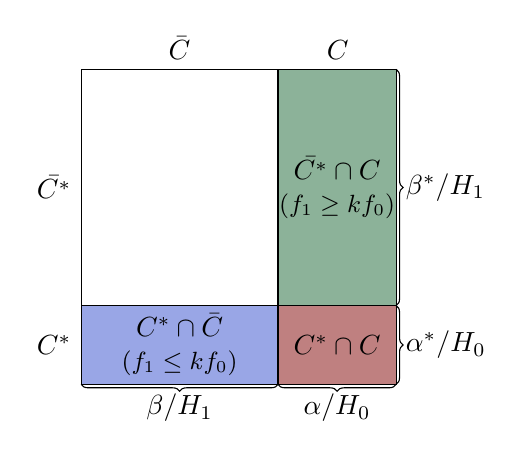
\begin{tikzpicture}
      \draw [fill=mblue!50!white] (0, 0) rectangle (2.5, 1);
      \draw [fill=mred!50!white] (2.5, 0) rectangle (4, 1);
      \draw (0, 1) rectangle (2.5, 4);
      \draw [fill=mgreen!50!white] (2.5, 1) rectangle (4, 4);

      \node at (0, 0.5) [left] {$C^*$};
      \node at (0, 2.5) [left] {$\bar{C^*}$};

      \node at (1.25, 4) [above] {$\bar{C}$};
      \node at (3.26, 4) [above] {$C$};

      \node [align=center] at (1.25, 0.5) {$C^*\cap \bar C$ \\\small $(f_1 \leq kf_0)$};
      \node [align=center] at (3.25, 2.5) {$\bar{C^*}\cap C$ \\\small $(f_1 \geq kf_0)$};
      \node [align=center] at (3.25, 0.5) {$C^*\cap C$};

      \draw [decorate, decoration={brace}] (2.5, 0) -- (0, 0) node [pos=0.5, below] {$\beta/H_1$};
      \draw [decorate, decoration={brace}] (4, 0) -- (2.5, 0) node [pos=0.5, below] {$\alpha/H_0$};

      \draw [decorate, decoration={brace}] (4, 1) -- (4, 0) node [pos=0.5, right] {$\alpha^*/H_0$};
      \draw [decorate, decoration={brace}] (4, 4) -- (4, 1) node [pos=0.5, right] {$\beta^*/H_1$};
    \end{tikzpicture}
  \end{center}
\end{proof}
Here we assumed the $f_0$ and $f_1$ are continuous densities. However, this assumption is need just to ensure that the likelihood ratio test of exactly size $\alpha$ exists. Even with non-continuous distributions, the likelihood ratio test is still a good idea. In fact, you will show in the example sheets that for a discrete distribution, as long as a likelihood ratio test of exactly size $\alpha$ exists, the same result holds.

\begin{eg}
  Suppose $X_1, \cdots, X_n$ are iid $N(\mu, \sigma_0^2)$, where $\sigma_0^2$ is known. We want to find the best size $\alpha$ test of $H_0: \mu = \mu_0$ against $H_1: \mu = \mu_1$, where $\mu_0$ and $\mu_1$ are known fixed values with $\mu_1 > \mu_0$. Then
  \begin{align*}
    \Lambda_\mathbf{x}(H_0; H_1) &= \frac{(2\pi\sigma_0^2)^{-n/2}\exp\left(-\frac{1}{2\sigma^2_0}\sum(x_i - \mu_1)^2\right)}{(2\pi\sigma_0^2)^{-n/2}\exp\left(-\frac{1}{2\sigma^2_0}\sum(x_i - \mu_0)^2\right)}\\
    &= \exp\left(\frac{\mu_1 - \mu_0}{\sigma_0^2}n\bar x + \frac{n(\mu_0^2 - \mu_1^2)}{2\sigma_0^2}\right).
  \end{align*}
  This is an increasing function of $\bar x$, so for any $k$, $\Lambda_x > k\Leftrightarrow \bar x > c$ for some $c$. Hence we reject $H_0$ if $\bar x > c$, where $c$ is chosen such that $\P(\bar X > c \mid H_0) = \alpha$.

  Under $H_0$, $\bar X \sim N(\mu_0, \sigma_0^2/n)$, so $Z = \sqrt{n}(\bar X - \mu_0)/\sigma_0 \sim N(0, 1)$.

  Since $\bar x > c\Leftrightarrow z > c'$ for some $c'$, the size $\alpha$ test rejects $H_0$ if
  \[
    z = \frac{\sqrt{n}(\bar x - \mu_0)}{\sigma_0} > z_\alpha.
  \]
  For example, suppose $\mu_0 = 5$, $\mu_1 = 6$, $\sigma_0 = 1$, $\alpha = 0.05$, $n = 4$ and $\mathbf{x} = (5.1, 5.5, 4.9, 5.3)$. So $\bar x = 5.2$.

  From tables, $z_{0.05} = 1.645$. We have $z = 0.4$ and this is less than $1.645$. So $\mathbf{x}$ is not in the rejection region.

  We do not reject $H_0$ at the 5\% level and say that the data are consistent with $H_0$.

  Note that this does not mean that we \emph{accept} $H_0$. While we don't have sufficient reason to believe it is false, we also don't have sufficient reason to believe it is true.

  This is called a $z$-\emph{test}.
\end{eg}

In this example, LR tests reject $H_0$ if $z > k$ for some constant $k$. The size of such a test is $\alpha = \P(Z > k\mid H_0) = 1 - \Phi(k)$, and is decreasing as $k$ increasing.
Our observed value $z$ will be in the rejected region iff $z > k \Leftrightarrow \alpha > p^* = \P(Z > z\mid H_0)$.
\begin{defi}[$p$-value]
  The quantity $p^*$ is called the \emph{$p$-value} of our observed data $\mathbf{x}$. For the example above, $z = 0.4$ and so $p^* = 1 - \Phi(0.4) = 0.3446$.
\end{defi}

In general, the $p$-value is sometimes called the ``observed significance level'' of $\mathbf{x}$. This is the probability under $H_0$ of seeing data that is ``more extreme'' than our observed data $\mathbf{x}$. Extreme observations are viewed as providing evidence against $H_0$.

\subsection{Composite hypotheses}
For composite hypotheses like $H:\theta \geq 0$, the error probabilities do not have a single value. We define
\begin{defi}[Power function]
  The \emph{power function} is
  \[
    W(\theta) = \P(\mathbf{X}\in C\mid \theta) = \P(\text{reject }H_0\mid \theta),
  \]
\end{defi}
We want $W(\theta)$ to be small on $H_0$ and large on $H_1$.

\begin{defi}[Size]
  The \emph{size} of the test is
  \[
    \alpha =\sup_{\theta\in \Theta_0}W(\theta),
  \]
\end{defi}
This is the worst possible size we can get.

For $\theta\in \Theta_1$, $1 - W(\theta) = \P(\text{Type II error}\mid \theta)$.

Sometimes the Neyman-Pearson theory can be extended to one-sided alternatives.

For example, in the previous example, we have shown that the most powerful size $\alpha$ test of $H_0: \mu = \mu_0$ versus $H_1: \mu = \mu_1$ (where $\mu_1 > \mu_0$) is given by
\[
  C = \left\{x: \frac{\sqrt{n}(\bar x - \mu_0)}{\sigma_0} > z_\alpha\right\}.
\]
The critical region depends on $\mu_0, n, \sigma_0, \alpha$, and the fact that $\mu_1 > \mu_0$. It does \emph{not} depend on the particular value of $\mu_1$. This test is then uniformly the most powerful size $\alpha$ for testing $H_0: \mu = \mu_0$ against $H_1: \mu> \mu_0$.

\begin{defi}[Uniformly most powerful test]
  A test specified by a critical region $C$ is \emph{uniformly most powerful} (UMP) size $\alpha$ test for test $H_0:\theta\in \Theta_0$ against $H_1: \theta \in \Theta_1$ if
  \begin{enumerate}
    \item $\sup_{\theta\in \Theta_0} W(\theta) = \alpha$.
    \item For any other test $C^*$ with size $\leq \alpha$ and with power function $W^*$, we have $W(\theta) \geq W^*(\theta)$ for all $\theta\in \Theta_1$.
  \end{enumerate}
  Note that these may not exist. However, the likelihood ratio test often works.
\end{defi}

\begin{eg}
  Suppose $X_1, \cdots, X_n$ are iid $N(\mu, \sigma_0^2)$ where $\sigma_0$ is known, and we wish to test $H_0: \mu\leq \mu_0$ against $H_1: \mu > \mu_0$.

  First consider testing $H_0': \mu = \mu_0$ against $H_1': \mu = \mu_1$, where $\mu_1 > \mu_0$. The Neyman-Pearson test of size $\alpha$ of $H_0'$ against $H_1'$ has
  \[
    C = \left\{x: \frac{\sqrt{n}(\bar x - \mu_0)}{\sigma_0} > z_\alpha\right\}.
  \]
  We show that $C$ is in fact UMP for the composite hypotheses $H_0$ against $H_1$. For $\mu\in \R$, the power function is
  \begin{align*}
    W(\mu) &= \P_\mu(\text{reject } H_0)\\
    &= \P_\mu\left(\frac{\sqrt{n}(\bar X - \mu_0)}{\sigma_0} > z_\alpha\right)\\
    &= \P_\mu\left(\frac{\sqrt{n}(\bar X - \mu)}{\sigma_0} > z_\alpha + \frac{\sqrt{n}(\mu_0 - \mu)}{\sigma_0}\right)\\
    &= 1 - \Phi\left(z_\alpha + \frac{\sqrt{n}(\mu_0 - \mu)}{\sigma_0}\right)
  \end{align*}
  To show this is UMP, we know that $W(\mu_0) = \alpha$ (by plugging in). $W(\mu)$ is an increasing function of $\mu$. So
  \[
    \sup_{ \mu \leq \mu_0} W(\mu) = \alpha.
  \]
  So the first condition is satisfied.

  For the second condition, observe that for any $\mu > \mu_0$, the Neyman Pearson size $\alpha$ test of $H_0'$ vs $H_1'$ has critical region $C$. Let $C^*$ and $W^*$ belong to any other test of $H_0$ vs $H_1$ of size $\leq \alpha$. Then $C^*$ can be regarded as a test of $H_0'$ vs $H_1'$ of size $\leq \alpha$, and the Neyman-Pearson lemma says that $W^*(\mu_1) \leq W(\mu_1)$. This holds for all $\mu_1 > \mu_0$. So the condition is satisfied and it is UMP.
\end{eg}
We now consider likelihood ratio tests for more general situations.
\begin{defi}[Likelihood of a composite hypothesis]
  The \emph{likelihood} of a composite hypothesis $H:\theta\in \Theta$ given data $\mathbf{x}$ to be
  \[
    L_{\mathbf{x}}(H) = \sup_{\theta\in \Theta}f(\mathbf{x}\mid \theta).
  \]
\end{defi}
So far we have considered disjoint hypotheses $\Theta_0, \Theta_1$, but we are not interested in any specific alternative. So it is easier to take $\Theta_1 = \Theta$ rather than $\Theta \setminus\Theta_0$. Then
\[
  \Lambda_\mathbf{x} (H_0; H_1) = \frac{L_\mathbf{x}(H_1)}{L_\mathbf{x}(H_0)}=\frac{\sup_{\theta\in \Theta_1}f(\mathbf{x}\mid \theta)}{\sup_{\theta\in \Theta_0}f(\mathbf{x}\mid \theta)} \geq 1,
\]
with large values of $\Lambda$ indicating departure from $H_0$.

\begin{eg}
  Single sample: testing a given mean, known variance ($z$-test). Suppose that $X_1, \cdots, X_n$ are iid $N(\mu, \sigma_0^2)$, with $\sigma_0^2$ known, and we wish to test $H_0: \mu = \mu_0$ against $H_1: \mu \not= \mu_0$ (for given constant $\mu_0$).

  Here $\Theta_0 = \{\mu_0\}$ and $\Theta = \R$.

  For the denominator, we have $\sup_\Theta f(\mathbf{x}\mid \mu) = f(\mathbf{x}\mid \hat{\mu})$, where $\hat{\mu}$ is the mle. We know that $\hat{\mu} = \bar x$. Hence
  \[
    \Lambda_\mathbf{x}(H_0; H_1) = \frac{(2\pi\sigma_0^2)^{-n/2}\exp\left(-\frac{1}{2\sigma^2_0}\sum(x_i - \bar x)^2\right)}{(2\pi\sigma_0^2)^{-n/2}\exp\left(-\frac{1}{2\sigma^2_0}\sum(x_i - \mu_0)^2\right)}.
  \]
  Then $H_0$ is rejected if $\Lambda_x$ is large.

  To make our lives easier, we can use the logarithm instead:
  \[
    2\log \Lambda(H_0;H_1) = \frac{1}{\sigma_0^2}\left[\sum (x_i - \mu_0)^2 - \sum (x_i - \bar x)^2\right] = \frac{n}{\sigma_0^2}(\bar x - \mu_0)^2.
  \]
  So we can reject $H_0$ if we have
  \[
    \left|\frac{\sqrt{n}(\bar x - \mu_0)}{\sigma_0}\right| > c
  \]
  for some $c$.

  We know that under $H_0$, $\displaystyle Z = \frac{\sqrt{n}(\bar X - \mu_0)}{\sigma_0}\sim N(0, 1)$. So the size $\alpha$ generalised likelihood test rejects $H_0$ if
  \[
    \left|\frac{\sqrt{n}(\bar x - \mu_0)}{\sigma_0}\right| > z_{\alpha/2}.
  \]
  Alternatively, since $\displaystyle \frac{n(\bar X - \mu_0)}{\sigma_0^2}\sim \chi_1^2$, we reject $H_0$ if
  \[
    \frac{n(\bar X - \mu_0)^2}{\sigma_0^2} > \chi_1^2(\alpha),
  \]
  (check that $z_{\alpha/2}^2 = \chi_1^2(\alpha)$).

  Note that this is a two-tailed test --- i.e.\ we reject $H_0$ both for high and low values of $\bar x$.
\end{eg}

The next theorem allows us to use likelihood ratio tests even when we cannot find the exact relevant null distribution.

First consider the ''size`` or ''dimension`` of our hypotheses: suppose that $H_0$ imposes $p$ independent restrictions on $\Theta$. So for example, if $\Theta = \{\theta: \theta = (\theta_1, \cdots, \theta_k)\}$, and we have
\begin{itemize}
  \item $H_0: \theta_{i_1} = a_1, \theta_{i_2} = a_2, \cdots \theta_{i_p} = a_p$; or
  \item $H_0: A\theta = \mathbf{b}$ (with $A$ $p\times k$, $\mathbf{b}$ $p\times 1$ given); or
  \item $H_0: \theta_i = f_i(\varphi), i = 1, \cdots, k$ for some $\varphi = (\varphi_1, \cdots, \varphi_{k - p})$.
\end{itemize}
We say $\Theta$ has $k$ free parameters and $\Theta_0$ has $k - p$ free parameters. We write $|\Theta_0| = k - p$ and $|\Theta| = k$.

\begin{thm}[Generalized likelihood ratio theorem]
  Suppose $\Theta_0 \subseteq \Theta_1$ and $|\Theta_1| - |\Theta_0| = p$. Let $\mathbf{X} = (X_1, \cdots, X_n)$ with all $X_i$ iid. Then if $H_0$ is true, as $n\to \infty$,
  \[
    2\log \Lambda_\mathbf{X}(H_0:H_1)\sim \chi_p^2.
  \]
  If $H_0$ is not true, then $2\log \Lambda$ tends to be larger. We reject $H_0$ if $2\log \Lambda > c$, where $c = \chi_p^2(\alpha)$ for a test of approximately size $\alpha$.
\end{thm}

For example, in our example above, $|\Theta_1| - |\Theta_0| = 1$, and in this case, we saw that under $H_0$, $2\log \Lambda \sim \chi_1^2$ \emph{exactly} for all $n$ in that particular case, rather than just approximately.

\subsection{Tests of goodness-of-fit and independence}
\subsubsection{Goodness-of-fit of a fully-specified null distribution}
So far, we have considered relatively simple cases where we are attempting to figure out, say, the mean. However, in reality, more complicated scenarios arise. For example, we might want to know if a dice is fair, i.e.\ if the probability of getting each number is exactly $\frac{1}{6}$. Our null hypothesis would be that $p_1 = p_2 = \cdots = p_6 = \frac{1}{6}$, while the alternative hypothesis allows any possible values of $p_i$.

In general, suppose the observation space $\mathcal{X}$ is partitioned into $k$ sets, and let $p_i$ be the probability that an observation is in set $i$ for $i = 1, \cdots, k$. We want to test ``$H_0:$ the $p_i$'s arise from a fully specified model'' against ``$H_1:$ the $p_i$'s are unrestricted (apart from the obvious $p_i \geq 0, \sum p_i = 1$)''.

\begin{eg}
  The following table lists the birth months of admissions to Oxford and Cambridge in 2012.
  \begin{center}
    \begin{tabular}{cccccccccccc}
      \toprule
      Sep & Oct & Nov & Dec & Jan & Feb & Mar & Apr & May & Jun & Jul & Aug\\
      470 & 515 & 470 & 457 & 473 & 381 & 466 & 457 & 437 & 396 & 384 & 394\\
      \bottomrule
    \end{tabular}
  \end{center}
  Is this compatible with a uniform distribution over the year?

  Out of $n$ independent observations, let $N_i$ be the number of observations in $i$th set. So $(N_1,\cdots, N_k)\sim \multinomial(n; p_1, \cdots, p_n)$.

  For a generalized likelihood ratio test of $H_0$, we need to find the maximised likelihood under $H_0$ and $H_1$.

  Under $H_1$, $\like(p_1, \cdots, p_k) \propto p_1^{n_1}\cdots p_k^{n_k}$. So the log likelihood is $l = \text{constant} + \sum n_i \log p_i$. We want to maximise this subject to $\sum p_i = 1$. Using the Lagrange multiplier, we will find that the mle is $\hat{p_i} = n_i/n$. Also $|\Theta_1| = k - 1$ (not $k$, since they must sum up to 1).

  Under $H_0$, the values of $p_i$ are specified completely, say $p_i = \tilde{p}_i$. So $|\Theta_0| = 0$. Using our formula for $\hat{p_i}$, we find that
  \[
    2\log \Lambda = 2\log\left(\frac{\hat{p}_1^{n_1}\cdots \hat{p}_k^{n_k}}{\tilde{p}_{1}^{n_1}\cdots \tilde{p}_k^{n_k}}\right) = 2\sum n_i \log \left(\frac{n_i}{n\tilde{p}_i}\right)\tag{1}
  \]
  Here $|\Theta_1| - |\Theta_0| = k - 1$. So we reject $H_0$ if $2\log \Lambda > \chi_{k - 1}^2(\alpha)$ for an approximate size $\alpha$ test.

  Under $H_0$ (no effect of month of birth), $\tilde{p}_i$ is the proportion of births in month $i$ in 1993/1994 --- this is \emph{not} simply proportional to the number of days in each month (or even worse, $\frac{1}{12}$), as there is for example an excess of September births (the ``Christmas effect''). So

  Then
  \[
    2\log \Lambda = 2\sum n_i \log\left(\frac{n_i}{n\tilde{p}_i}\right) = 44.9.
  \]
  $\P(\chi_{11}^2 > 44.86) = 3\times 10^{-9}$, which is our $p$-value. Since this is certainly less than 0.001, we can reject $H_0$ at the $0.1\%$ level, or can say the result is ``significant at the $0.1\%$ level''.

  The traditional levels for comparison are $\alpha = 0.04, 0.01, 0.001$, roughly corresponding to ``evidence'', ``strong evidence'' and ``very strong evidence''.
\end{eg}
A similar common situation has $H_0: p_i = p_i(\theta)$ for some parameter $\theta$ and $H_1$ as before. Now $|\Theta_0|$ is the number of independent parameters to be estimated under $H_0$.

Under $H_0$, we find mle $\hat{\theta}$ by maximizing $n_i \log p_i (\theta)$, and then
\[
  2\log \Lambda = 2\log \left(\frac{\hat{p_1}^{n_1}\cdots \hat{p_k}^{n_k}}{p_1(\hat{\theta})^{n_1}\cdots p_k (\hat{\theta})^{n_1}}\right) = 2\sum n_i \log \left(\frac{n_i}{np_i(\hat{\theta})}\right).\tag{2}
\]
The degrees of freedom are $k - 1 - |\Theta_0|$.

\subsubsection{Pearson's Chi-squared test}
Notice that the two log likelihoods are of the same form. In general, let $o_i = n_i$ (observed number) and let $e_i = n\tilde{p_i}$ or $np_i(\hat{\theta})$ (expected number). Let $\delta_i = o_i - e_i$. Then
\begin{align*}
  2\log \Lambda &= 2\sum o_i \log \left(\frac{o_i}{e_i}\right)\\
  &= 2\sum (e_i + \delta_i) \log\left(1 + \frac{\delta_i}{e_i}\right)\\
  &= 2\sum (e_i + \delta_i) \left(\frac{\delta_i}{e_i} - \frac{\delta_i^2}{2e_i^2} + O(\delta_i^3)\right)\\
  &= 2\sum \left(\delta_i + \frac{\delta_i^2}{e_i} - \frac{\delta_i^2}{2e_i} + O(\delta_i^3)\right)\\
  \intertext{We know that $\sum \delta_i = 0$ since $\sum e_i = \sum o_i$. So}
  &\approx \sum \frac{\delta_i^2}{e_i}\\
  &= \sum\frac{(o_i - e_i)^2}{e_i}.
\end{align*}
This is known as the \emph{Pearson's Chi-squared test}.

\begin{eg}
  Mendel crossed 556 smooth yellow male peas with wrinkled green peas. From the progeny, let
  \begin{enumerate}
    \item $N_1$ be the number of smooth yellow peas,
    \item $N_2$ be the number of smooth green peas,
    \item $N_3$ be the number of wrinkled yellow peas,
    \item $N_4$ be the number of wrinkled green peas.
  \end{enumerate}
  We wish to test the goodness of fit of the model
  \begin{center}
    $H_0: (p_1, p_2, p_3, p_4) = \left(\frac{9}{16}, \frac{3}{16}, \frac{3}{16}, \frac{1}{16}\right)$.
  \end{center}
  Suppose we observe $(n_1, n_2, n_3, n_4) = (315, 108, 102, 31)$.

  We find $(e_1, e_2, e_3, e_4) = (312.75, 104.25, 104.25, 34.75)$. The actual $2\log \Lambda = 0.618$ and the approximation we had is $\sum \frac{(o_i - e_i)^2}{e_i} = 0.604$.

  Here $|\Theta_0| = 0$ and $|\Theta_1| = 4 - 1 = 3$. So we refer to test statistics $\chi_3^2(\alpha)$.

  Since $\chi_3^2(0.05) = 7.815$, we see that neither value is significant at $5\%$. So there is no evidence against Mendel's theory. In fact, the $p$-value is approximately $\P(\chi_3^2 > 0.6) \approx 0.96$. This is a \emph{really} good fit, so good that people suspect the numbers were not genuine.
\end{eg}

\begin{eg}
  In a genetics problem, each individual has one of the three possible genotypes, with probabilities $p_1, p_2, p_3$. Suppose we wish to test $H_0: p_i = p_i(\theta)$, where
  \[
    p_1(\theta) = \theta^2,\quad p_2 = 2\theta(1 - \theta), \quad p_3(\theta) = (1 - \theta)^2.
  \]
  for some $\theta \in (0, 1)$.

  We observe $N_i = n_i$. Under $H_0$, the mle $\hat{\theta}$ is found by maximising
  \[
    \sum n_i \log p_i(\theta) = 2n_1 \log \theta + n_2\log(2\theta(1 - \theta)) + 2n_3 \log (1 - \theta).
  \]
  We find that $\hat{\theta} = \frac{2n_1 + n_2}{2n}$. Also, $|\Theta_0| = 1$ and $|\Theta_1| = 2$.

  After conducting an experiment, we can substitute $p_i(\hat{\theta})$ into (2), or find the corresponding Pearson's chi-squared statistic, and refer to $\chi_1^2$.
\end{eg}

\subsubsection{Testing independence in contingency tables}
\begin{defi}[Contingency table]
  A \emph{contingency table} is a table in which observations or individuals are classified according to one or more criteria.
\end{defi}

\begin{eg}
  500 people with recent car changes were asked about their previous and new cars. The results are as follows:
  \begin{center}
    \begin{tabular}{ccccc}
      \toprule
      & & & New car &\\
      & & Large & Medium & Small\\\midrule
      \multirow{3}{*}{\rotatebox[origin=c]{90}{Previous}\;\rotatebox[origin=c]{90}{car}}& Large & 56 & 52 & 42\\
      & Medium & 50 & 83 & 67\\
      & Small & 18 & 51 & 81\\\bottomrule
    \end{tabular}
  \end{center}
  This is a two-way contingency table: Each person is classified according to the previous car size and new car size.
\end{eg}
Consider a two-way contingency table with $r$ rows and $c$ columns. For $i = 1, \cdots, r$ And $j = 1, \cdots, c$, let $p_{ij}$ be the probability that an individual selected from the population under consideration is classified in row $i$ and column $j$. (i.e.\ in the $(i, j)$ cell of the table).

Let $p_{i+} = \P(\text{in row }i)$ and $p_{+j} = \P(\text{in column }j)$. Then we must have $p_{++} = \sum_i \sum_j p_{ij} = 1$.

Suppose a random sample of $n$ individuals is taken, and let $n_{ij}$ be the number of these classified in the $(i, j)$ cell of the table.

Let $n_{i+} = \sum_j n_{ij}$ and $n_{+j} = \sum_i n_{ij}$. So $n_{++} = n$.

We have
\[
  (N_{11}, \cdots, N_{1c}, N_{21}, \cdots, N_{rc}) \sim \multinomial (n; p_{11}, \cdots, p_{1c}, p_{21}, \cdots, p_{rc}).
\]
We may be interested in testing the null hypothesis that the two classifications are independent. So we test
\begin{itemize}
  \item $H_0$: $p_i = p_{i+}p_{+j}$ for all $i, j$, i.e.\ independence of columns and rows.
  \item $H_1$: $p_{ij}$ are unrestricted.
\end{itemize}
Of course we have the usual restrictions like $p_{++} = 1$, $p_{ij} \geq 0$.

Under $H_1$, the mles are $\hat{p_{ij}} = \frac{n_{ij}}{n}$.

Under $H_0$, the mles are $\hat{p}_{i+} = \frac{n_{i+}}{n}$ and $\hat{p}_{+j} = \frac{n_{+j}}{n}$.

Write $o_{ij} = n_{ij}$ and $e_{ij} = n\hat{p}_{i+}\hat{p}_{+j} = n_{i+}n_{+j}/n$.

Then
\[
  2\log \Lambda = 2\sum_{i = 1}^r \sum_{j = 1}^c o_{ij}\log\left(\frac{o_{ij}}{e_{ij}}\right) \approx \sum_{i = 1}^r \sum_{j = 1}^c \frac{(o_{ij} - e_{ij})^2}{e_{ij}}.
\]
using the same approximating steps for Pearson's Chi-squared test.

We have $|\Theta_1| = rc - 1$, because under $H_1$ the $p_{ij}$'s sum to one. Also, $|\Theta_0| = (r - 1) + (c - 1)$ because $p_{1+}, \cdots, p_{r+}$ must satisfy $\sum_i p_{i+} = 1$ and $p_{+1}, \cdots, p_{+c}$ must satisfy $\sum_j p_{+j} = 1$. So
\[
  |\Theta_1| - |\Theta_0| = rc - 1 - (r - 1) - (c - 1) = (r - 1)(c - 1).
\]

\begin{eg}
  In our previous example, we wish to test $H_0$: the new and previous car sizes are independent. The actual data is:
  \begin{center}
    \begin{tabular}{cccccc}
      \toprule
      & & & New car &\\
      & & Large & Medium & Small & \textbf{Total}\\\midrule
      \multirow{4}{*}{\rotatebox[origin=c]{90}{Previous}\;\rotatebox[origin=c]{90}{car}}& Large & 56 & 52 & 42 & \textbf{150}\\
      & Medium & 50 & 83 & 67 & \textbf{120}\\
      & Small & 18 & 51 & 81 & \textbf{150}\\\cmidrule{2-6}
      & \textit{Total} & \textit{124} & \textit{186} & \textit{190} & \textit{\textbf{500}}\\\bottomrule
    \end{tabular}
  \end{center}
  while the expected values given by $H_0$ is
  \begin{center}
    \begin{tabular}{cccccc}
      \toprule
      & & & New car &\\
      & & Large & Medium & Small & \textbf{Total}\\\midrule
      \multirow{4}{*}{\rotatebox[origin=c]{90}{Previous}\;\rotatebox[origin=c]{90}{car}}& Large & 37.2 & 55.8 & 57.0 & \textbf{150}\\
      & Medium & 49.6 & 74.4 & 76.0 & \textbf{120}\\
      & Small & 37.2 & 55.8 & 57.0 & \textbf{150}\\\cmidrule{2-6}
      & \textit{Total} & \textit{124} & \textit{186} & \textit{190} & \textit{\textbf{500}}\\\bottomrule
    \end{tabular}
  \end{center}
  Note the margins are the same. It is quite clear that they do not match well, but we can find the $p$ value to be sure.

  $\displaystyle\sum\sum \frac{(o_{ij} - e_{ij})^2}{e_{ij}} = 36.20$, and the degrees of freedom is $(3 - 1)(3 - 1) = 4$.

  From the tables, $\chi_4^2(0.05) = 9.488$ and $\chi_4^2(0.01) = 13.28$.

  So our observed value of 36.20 is significant at the $1\%$ level, i.e.\ there is strong evidence against $H_0$. So we conclude that the new and present car sizes are not independent.
\end{eg}
\subsection{Tests of homogeneity, and connections to confidence intervals}
\subsubsection{Tests of homogeneity}
\begin{eg}
  150 patients were randomly allocated to three groups of 50 patients each. Two groups were given a new drug at different dosage levels, and the third group received a placebo. The responses were as shown in the table below.
  \begin{center}
    \begin{tabular}{ccccc}
      \toprule
      & Improved & No difference & Worse & \textbf{Total}\\\midrule
      Placebo & 18 & 17 & 15 & \textbf{50}\\
      Half dose & 20 & 10 & 20 & \textbf{50}\\
      Full dose & 25 & 13 & 12& \textbf{50}\\\midrule
      \textit{Total} & \textit{63} & \textit{40} & \textit{47} & \textbf{\textit{150}}\\\bottomrule
    \end{tabular}
  \end{center}
  Here the row totals are fixed in advance, in contrast to our last section, where the row totals are random variables.

  For the above, we may be interested in testing $H_0:$ the probability of ``improved'' is the same for each of the three treatment groups, and so are the probabilities of ``no difference'' and ``worse'', i.e.\ $H_0$ says that we have homogeneity down the rows.
\end{eg}
In general, we have independent observations from $r$ multinomial distributions, each of which has $c$ categories, i.e.\ we observe an $r\times c$ table $(n_{ij})$, for $i = 1, \cdots, r$ and $j = 1, \cdots, c$, where
\[
  (N_{i1}, \cdots, N_{ic}) \sim \multinomial(n_{i+}, p_{i1}, \cdots, p_{ic})
\]
independently for each $i = 1, \cdots, r$.
We want to test
\[
  H_0: p_{1j} = p_{2j} = \cdots = p_{rj} = p_j,
\]
for $j = 1, \cdots, c$, and
\[
  H_1: p_{ij}\text{ are unrestricted}.
\]
Using $H_1$,
\[
  \like(p_{ij}) = \prod_{i = 1}^r \frac{n_{i+}!}{n_{i1}!\cdots n_{ic}!}p_{i1}^{n_{i1}} \cdots p_{ic}^{n_{ic}},
\]
and
\[
  \log\like = \text{constant} + \sum_{i = 1}^r \sum_{j = 1}^c n_{ij}\log p_{ij}.
\]
Using Lagrangian methods, we find that $\hat{p}_{ij} = \frac{n_{ij}}{n_{i+}}$.

Under $H_0$,
\[
  \log\like = \text{constant} + \sum_{j = 1}^c n_{+j}\log p_j.
\]
By Lagrangian methods, we have $\hat{p}_j = \frac{n_{+j}}{n_{++}}$.

Hence
\[
  2\log \Lambda = \sum_{i = 1}^{r}\sum_{j = 1}^c n_{ij}\log\left(\frac{\hat{p}_{ij}}{\hat{p}_j}\right) = 2\sum_{i = 1}^r\sum_{j = 1}^c n_{ij}\log\left(\frac{n_{ij}}{n_{i+}n_{+j}/n_{++}}\right),
\]
which is the same as what we had last time, when the row totals are unrestricted!

We have $|\Theta_1| = r(c - 1)$ and $|\Theta_0| = c - 1$. So the degrees of freedom is $r(c - 1) - (c - 1) = (r - 1)(c - 1)$, and under $H_0$, $2\log\Lambda$ is approximately $\chi^2_{(r - 1)(c - 1)}$. Again, it is exactly the same as what we had last time!

We reject $H_0$ if $2\log \Lambda > \chi_{(r - 1)(c - 1)}^2 (\alpha)$ for an approximate size $\alpha$ test.

If we let $o_{ij}= n_{ij}, e_{ij} = \frac{n_{i+}n_{+j}}{n_{++}}$, and $\delta_{ij} = o_{ij} - e_{ij}$, using the same approximating steps as for Pearson's Chi-squared, we obtain
\[
  2\log \Lambda \approx \sum \frac{(o_{ij} - e_{ij})^2}{e_{ij}}.
\]
\begin{eg}
  Continuing our previous example, our data is
  \begin{center}
    \begin{tabular}{ccccc}
      \toprule
      & Improved & No difference & Worse & \textbf{Total}\\\midrule
      Placebo & 18 & 17 & 15 & \textbf{50} \\
      Half dose & 20 & 10 & 20 & \textbf{50} \\
      Full dose & 25 & 13 & 12& \textbf{50} \\\midrule
      \textit{Total} & \textit{6}3 & \textit{40} & \textit{47} & \textbf{\textit{150}} \\ \bottomrule
    \end{tabular}
  \end{center}
  The expected under $H_0$ is
  \begin{center}
    \begin{tabular}{ccccc}
      \toprule
      & Improved & No difference & Worse &\textbf{Total}\\\midrule
      Placebo & 21 & 13.3 & 15.7 & \textbf{50} \\
      Half dose & 21 & 13.3 & 15.7 & \textbf{50}\\
      Full dose & 21 & 13.3 & 15.7 & \textbf{50}\\\midrule
      \textit{Total}& \textit{63} & \textit{40} & \textit{47} & \textbf{\textit{150}}\\ \bottomrule
    \end{tabular}
  \end{center}
  We find $2\log \Lambda = 5.129$, and we refer this to $\chi_4^2$. Clearly this is not significant, as the mean of $\chi_4^2$ is $4$, and is something we would expect to happen solely by chance.

  We can calculate the $p$-value: from tables, $\chi_4^2(0.05) = 9.488$, so our observed value is not significant at $5\%$, and the data are consistent with $H_0$.

  We conclude that there is no evidence for a difference between the drug at the given doses and the placebo.

  For interest,
  \[
    \sum\frac{(o_{ij} - e_{ij})^2}{e_{ij}} = 5.173,
  \]
  giving the same conclusion.
\end{eg}
\subsubsection{Confidence intervals and hypothesis tests}
Confidence intervals or sets can be obtained by inverting hypothesis tests, and vice versa

\begin{defi}[Acceptance region]
  The \emph{acceptance region} $A$ of a test is the complement of the critical region $C$.

  Note that when we say ``acceptance'', we really mean ``non-rejection''! The name is purely for historical reasons.
\end{defi}
Suppose $X_1, \cdots, X_n$ have joint pdf $f_\mathbf{X}(\mathbf{x}\mid \theta)$ for $\theta\in \Theta$

\begin{thm}\leavevmode
  \begin{enumerate}
    \item Suppose that for every $\theta_0\in \Theta$ there is a size $\alpha$ test of $H_0: \theta = \theta_0$. Denote the acceptance region by $A(\theta_0)$. Then the set $I(\mathbf{X}) = \{\theta:\mathbf{X}\in A(\theta)\}$ is a $100(1 - \alpha)\%$ confidence set for $\theta$.
    \item Suppose $I(\mathbf{X})$ is a $100(1 - \alpha)\%$ confidence set for $\theta$. Then $A(\theta_0) = \{\mathbf{X}: \theta_0 \in I(\mathbf{X})\}$ is an acceptance region for a size $\alpha$ test of $H_0: \theta = \theta_0$.
  \end{enumerate}
\end{thm}
Intuitively, this says that ``confidence intervals'' and ``hypothesis acceptance/rejection'' are the same thing. After gathering some data $\mathbf{X}$, we can produce a, say, $95\%$ confidence interval $(a, b)$. Then if we want to test the hypothesis $H_0: \theta = \theta_0$, we simply have to check whether $\theta_0 \in (a, b)$.

On the other hand, if we have a test for $H_0: \theta = \theta_0$, then the confidence interval is all $\theta_0$ in which we would accept $H_0: \theta = \theta_0$.
\begin{proof}
  First note that $\theta_0\in I(\mathbf{X})$ iff $\mathbf{X}\in A(\theta_0)$.

  For (i), since the test is size $\alpha$, we have
  \[
    \P(\text{accept }H_0\mid H_0\text{ is true}) = \P(\mathbf{X}\in A_(\theta_0)\mid \theta=\theta_0) = 1 - \alpha.
  \]
  And so
  \[
    \P(\theta_0\in I(\mathbf{X})\mid \theta = \theta_0) = \P(\mathbf{X}\in A(\theta_0)\mid \theta = \theta_0) = 1 - \alpha.
  \]
  For (ii), since $I(\mathbf{X})$ is a $100(1 - \alpha)\%$ confidence set, we have
  \[
    P(\theta_0\in I(\mathbf{X})\mid \theta = \theta_0) = 1- \alpha.
  \]
  So
  \[
    \P(\mathbf{X}\in A(\theta_0)\mid \theta = \theta_0) = \P(\theta\in I(\mathbf{X})\mid \theta = \theta_0) = 1- \alpha.\qedhere
  \]
\end{proof}

\begin{eg}
  Suppose $X_1, \cdots, X_n$ are iid $N(\mu, 1)$ random variables and we want a $95\%$ confidence set for $\mu$.

  One way is to use the theorem and find the confidence set that belongs to the hypothesis test that we found in the previous example. We find a test of size 0.05 of $H_0 : \mu= \mu_0$ against $H_1: \mu\not= \mu_0$ that rejects $H_0$ when $|\sqrt{n}(\bar x - \mu_0)| > 1.96$ (where 1.96 is the upper $2.5\%$ point of $N(0, 1)$).

  Then $I(\mathbf{X}) = \{\mu: \mathbf{X}\in A(\mu)\} = \{\mu:|\sqrt{n}(\bar X - \mu)| < 1.96\%\}$. So a $95\%$ confidence set for $\mu$ is $(\bar X - 1.96/\sqrt{n}, \bar X + 1.96/\sqrt{n})$.
\end{eg}
\subsection{Multivariate normal theory}
\subsubsection{Multivariate normal distribution}
So far, we have only worked with scalar random variables or a vector of iid random variables. In general, we can have a random (column) vector $\mathbf{X} = (X_1, \cdots, X_n)^T$, where the $X_i$ are correlated.

The mean of this vector is given by
\[
  \boldsymbol\mu = \E[\mathbf{X}] = (\E(X_1), \cdots, \E(X_n))^T = (\mu_1, \cdots, \mu_n)^T.
\]
Instead of just the variance, we have the covariance matrix
\[
  \cov (\mathbf{X}) = \E[(\mathbf{X} - \boldsymbol\mu)(\mathbf{X} - \boldsymbol\mu)^T] = (\cov(X_i, X_j))_{ij},
\]
provided they exist, of course.

We can multiply the vector $\mathbf{X}$ by an $m\times n$ matrix $A$. Then we have
\[
  \E[A\mathbf{X}] = A\boldsymbol\mu,
\]
and
\[
  \cov (A\mathbf{X}) = A\cov(\mathbf{X})A^T.\tag{$*$}
\]
The last one comes from
\begin{align*}
  \cov(A\mathbf{X}) &= \E[(A\mathbf{X} -\E[A\mathbf{X}])(A\mathbf{X} - \E[A\mathbf{X}])^T] \\
  &= \E[A(\mathbf{X} - \E\mathbf{X})(\mathbf{X} - \E\mathbf{X})^T A^T]\\
  &= A\E[(\mathbf{X} - \E\mathbf{X})(\mathbf{X} - \E\mathbf{X})^T]A^T.
\end{align*}
If we have two random vectors $\mathbf{V}, \mathbf{W}$, we can define the covariance $\cov(\mathbf{V}, \mathbf{W})$ to be a matrix with $(i, j)$th element $\cov(V_i, W_j)$. Then $\cov(A\mathbf{X}, B\mathbf{X}) = A\cov (\mathbf{X}) B^T$.

An important distribution is a \emph{multivariate normal distribution}.

\begin{defi}[Multivariate normal distribution]
  $\mathbf{X}$ has a \emph{multivariate normal distribution} if, for every $\mathbf{t}\in \R^n$, the random variable $\mathbf{t}^T\mathbf{X}$ (i.e.\ $\mathbf{t}\cdot \mathbf{X}$) has a normal distribution. If $\E[\mathbf{X}] = \boldsymbol\mu$ and $\cov (\mathbf{X}) = \Sigma$, we write $\mathbf{X}\sim N_n(\boldsymbol\mu, \Sigma)$.
\end{defi}

Note that $\Sigma$ is symmetric and is positive semi-definite because by $(*)$,
\[
  \mathbf{t}^T\Sigma \mathbf{t} = \var(\mathbf{t}^T\mathbf{X}) \geq 0.
\]
So what is the pdf of a multivariate normal? And what is the moment generating function? Recall that a (univariate) normal $X\sim N(\mu, \sigma^2)$ has density
\[
  f_X(x; \mu, \sigma^2) = \frac{1}{\sqrt{2\pi}\sigma} \exp\left(-\frac{1}{2}\frac{(x - \mu)^2}{\sigma^2}\right),
\]
with moment generating function
\[
  M_X(s) = \E[e^{sX}] = \exp\left(\mu s + \frac{1}{2}\sigma^2 s^2\right).
\]
Hence for any $\mathbf{t}$, the moment generating function of $\mathbf{t}^T\mathbf{X}$ is given by
\[
  M_{\mathbf{t}^T \mathbf{X}}(s) = \E[e^{s\mathbf{t}^T\mathbf{X}}] = \exp\left(\mathbf{t}^T\boldsymbol\mu s + \frac{1}{2}\mathbf{t}^T\Sigma \mathbf{t}s^2\right).
\]
Hence $\mathbf{X}$ has mgf
\[
  M_\mathbf{X}(\mathbf{t}) = \E[e^{\mathbf{t}^T \mathbf{X}}]= M_{\mathbf{t}^T\mathbf{X}}(1) = \exp\left(\mathbf{t}^T\boldsymbol\mu + \frac{1}{2}\mathbf{t}^T \Sigma \mathbf{t}\right).\tag{$\dagger$}
\]

\begin{prop}\leavevmode
  \begin{enumerate}
    \item If $\mathbf{X} \sim N_n(\mu, \Sigma)$, and $A$ is an $m\times n$ matrix, then $A\mathbf{X} \sim N_m (A\boldsymbol\mu, A\Sigma A^T)$.
    \item If $\mathbf{X}\sim N_n(\mathbf{0}, \sigma^2 I)$, then
      \[
        \frac{|\mathbf{X}|^2}{\sigma^2} = \frac{\mathbf{X}^T\mathbf{X}}{\sigma^2} = \sum \frac{X_i^2}{\sigma ^2}\sim \chi_n^2.
      \]
      Instead of writing $|\mathbf{X}|^2/\sigma^2 \sim \chi_n^2$, we often just say $|\mathbf{X}|^2 \sim \sigma^2 \chi_n^2$.
  \end{enumerate}
\end{prop}

\begin{proof}\leavevmode
  \begin{enumerate}
    \item See example sheet 3.
    \item Immediate from definition of $\chi_n^2$.\qedhere
  \end{enumerate}
\end{proof}

\begin{prop}
  Let $\mathbf{X}\sim N_n(\mu, \Sigma)$. We split $\mathbf{X}$ up into two parts: $\mathbf{X} =
  \begin{pmatrix}
    \mathbf{X}_1\\
    \mathbf{X}_2
  \end{pmatrix}$, where $\mathbf{X}_i$ is a $n_i \times 1$ column vector and $n_1 + n_2 = n$.

  Similarly write
  \[
    \boldsymbol\mu =
    \begin{pmatrix}
      \boldsymbol\mu_1\\
      \boldsymbol\mu_2
    \end{pmatrix}
    ,\quad
    \Sigma =
    \begin{pmatrix}
      \Sigma_{11} & \Sigma_{12}\\
      \Sigma_{21} & \Sigma_{22}
    \end{pmatrix},
  \]
  where $\Sigma_{ij}$ is an $n_i\times n_j$ matrix.

  Then
  \begin{enumerate}
    \item $\mathbf{X}_i \sim N_{n_i}(\boldsymbol\mu_i, \Sigma_{ii})$
    \item $\mathbf{X}_1$ and $\mathbf{X}_2$ are independent iff $\Sigma_{12} = 0$.
  \end{enumerate}
\end{prop}

\begin{proof}\leavevmode
  \begin{enumerate}
    \item See example sheet 3.
    \item Note that by symmetry of $\Sigma$, $\Sigma_{12} = 0$ if and only if $\Sigma_{21} = 0$.

      From $(\dagger)$, $M_\mathbf{X}(\mathbf{t}) = \exp(\mathbf{t}^T \boldsymbol\mu + \frac{1}{2}\mathbf{t}^T\Sigma\mathbf{t})$ for each $\mathbf{t}\in \R^n$. We write $\mathbf{t} = \begin{pmatrix}\mathbf{t}_1\\\mathbf{t}_2\end{pmatrix}$. Then the mgf is equal to
      \[
        M_\mathbf{X}(\mathbf{t}) = \exp\left(\mathbf{t}_1^T\boldsymbol\mu_1 + \mathbf{t}_2^T \Sigma_{11}\mathbf{t}_1 + \frac{1}{2}\mathbf{t}_2^T \Sigma_{22}\mathbf{t}_2 + \frac{1}{2}\mathbf{t}_1^T \Sigma_{12}\mathbf{t}_2 + \frac{1}{2}\mathbf{t}_2^T \Sigma_{21}\mathbf{t}_1\right).
      \]
      From (i), we know that $M_{\mathbf{X}_i}(\mathbf{t}_i) = \exp(\mathbf{t}_i^T\boldsymbol\mu_i + \frac{1}{2}\mathbf{t}_i^T \Sigma_{ii}\mathbf{t}_i)$. So $M_\mathbf{X}(\mathbf{t}) = M_{\mathbf{X}_1}(\mathbf{t}_1)M_{\mathbf{X}_2}(\mathbf{t}_2)$ for all $\mathbf{t}$ if and only if $\Sigma_{12} = 0$.\qedhere
  \end{enumerate}
\end{proof}

\begin{prop}
  When $\Sigma$ is a positive definite, then $\mathbf{X}$ has pdf
  \[
    f_\mathbf{X}(\mathbf{x}; \mu, \Sigma) = \frac{1}{|\Sigma|^2} \left(\frac{1}{\sqrt{2\pi}}\right)^n \exp\left[-\frac{1}{2}(\mathbf{x} - \boldsymbol\mu)^T\Sigma^{-1}(\mathbf{x} - \boldsymbol\mu)\right].
  \]
\end{prop}
Note that $\Sigma$ is always positive semi-definite. The conditions just forbid the case $|\Sigma| = 0$, since this would lead to dividing by zero.

\subsubsection{Normal random samples}
We wish to use our knowledge about multivariate normals to study univariate normal data. In particular, we want to prove the following:

\begin{thm}[Joint distribution of $\bar X$ and $S_{XX}$]
  Suppose $X_1, \cdots, X_n$ are iid $N(\mu, \sigma^2)$ and $\bar X = \frac{1}{n} \sum X_i$, and $S_{XX} = \sum (X_i - \bar X)^2$. Then
  \begin{enumerate}
    \item $\bar X \sim N(\mu, \sigma^2/n)$
    \item $S_{XX}/\sigma^2 \sim \chi_{n - 1}^2$.
    \item $\bar X$ and $S_{XX}$ are independent.
  \end{enumerate}
\end{thm}

\begin{proof}
  We can write the joint density as $\mathbf{X} \sim N_n(\boldsymbol\mu, \sigma^2I)$, where $\boldsymbol\mu = (\mu, \mu, \cdots, \mu)$.

  Let $A$ be an $n\times n$ orthogonal matrix with the first row all $1/\sqrt{n}$ (the other rows are not important). One possible such matrix is
  \[
    A =
    \begin{pmatrix}
      \frac{1}{\sqrt{n}} & \frac{1}{\sqrt{n}} & \frac{1}{\sqrt{n}} & \frac{1}{\sqrt{n}} & \cdots & \frac{1}{\sqrt{n}}\\
      \frac{1}{\sqrt{2\times 1}} & \frac{-1}{\sqrt{2\times 1}} & 0 & 0 & \cdots & 0\\
      \frac{1}{\sqrt{3\times 2}} & \frac{1}{\sqrt{3\times 2}} & \frac{-2}{\sqrt{3\times 2}} & 0 & \cdots & 0\\
      \vdots & \vdots & \vdots & \vdots & \ddots & \vdots \\
      \frac{1}{\sqrt{n(n - 1)}} & \frac{1}{\sqrt{n(n - 1)}} & \frac{1}{\sqrt{n(n - 1)}} & \frac{1}{\sqrt{n(n - 1)}} & \cdots & \frac{-(n - 1)}{\sqrt{n(n - 1)}} \\
    \end{pmatrix}
  \]
  Now define $\mathbf{Y} = A\mathbf{X}$. Then
  \[
    \mathbf{Y} \sim N_n(A\boldsymbol\mu, A\sigma^2IA^T) = N_n(A\boldsymbol\mu, \sigma^2 I).
  \]
  We have
  \[
    A\boldsymbol\mu = (\sqrt{n}\mu, 0, \cdots, 0)^T.
  \]
  So $Y_1 \sim N(\sqrt{n}\mu, \sigma^2)$ and $Y_i \sim N(0, \sigma^2)$ for $i = 2, \cdots, n$. Also, $Y_1, \cdots, Y_n$ are independent, since the covariance matrix is every non-diagonal term $0$.

  But from the definition of $A$, we have
  \[
    Y_1 = \frac{1}{\sqrt{n}}\sum_{i = 1}^n X_i = \sqrt{n} \bar X.
  \]
  So $\sqrt{n} \bar X \sim N(\sqrt{n}\mu, \sigma^2)$, or $\bar X \sim N(\mu, \sigma^2/n)$. Also
  \begin{align*}
    Y_2^2 + \cdots + Y_n^2 &= \mathbf{Y}^T\mathbf{Y} - Y_1^2\\
    &= \mathbf{X}^TA^TA\mathbf{X} - Y_1^2\\
    &= \mathbf{X}^T\mathbf{X} - n\bar X^2\\
    &= \sum_{i = 1}^n X_i^2 - n\bar X^2\\
    &= \sum_{i = 1}^n (X_i - \bar X)^2 \\
    &= S_{XX}.
  \end{align*}
  So $S_{XX} = Y_2^2 + \cdots + Y^2_n \sim \sigma^2 \chi_{n - 1}^2$.

  Finally, since $Y_1$ and $Y_2, \cdots, Y_n$ are independent, so are $\bar X$ and $S_{XX}$.
\end{proof}
\subsection{Student's \texorpdfstring{$t$}{t}-distribution}
\begin{defi}[$t$-distribution]
  Suppose that $Z$ and $Y$ are independent, $Z\sim N(0, 1)$ and $Y\sim \chi_k^2$. Then
  \[
    T = \frac{Z}{\sqrt{Y/k}}
  \]
  is said to have a $t$-distribution on $k$ degrees of freedom, and we write $T\sim t_k$.
\end{defi}

The density of $t_k$ turns out to be
\[
  f_T(t) = \frac{\Gamma((k + 1)/2)}{\Gamma(k/2)} \frac{1}{\sqrt{\pi k}}\left(1 + \frac{t^2}{k}\right)^{-(k+1)/2}.
\]
This density is symmetric, bell-shaped, and has a maximum at $t = 0$, which is rather like the standard normal density. However, it can be shown that $\P(T > t) > \P(Z > t)$, i.e.\ the $T$ distribution has a ``fatter'' tail. Also, as $k \to \infty$, $t_k$ approaches a normal distribution.

\begin{prop}
  If $k > 1$, then $\E_k(T) = 0$.

  If $k > 2$, then $\var_k(T) = \frac{k}{k - 2}$.

  If $k = 2$, then $\var_k(T) = \infty$.

  In all other cases, the values are undefined. In particular, the $k = 1$ case, this is known as the Cauchy distribution, and has undefined mean and variance.
\end{prop}

\begin{notation}
  We write $t_k(\alpha)$ be the upper $100\alpha\%$ point of the $t_k$ distribution, so that $\P(T > t_k(\alpha)) = \alpha$.
\end{notation}

Why would we define such a weird distribution? The typical application is to study random samples with unknown mean \emph{and} unknown variance.

Let $X_1, \cdots, X_n$ be iid $\N(\mu, \sigma^2)$. Then $\bar X \sim N(\mu, \sigma^2/n)$. So $Z = \frac{\sqrt{n}(\bar X - \mu)}{\sigma} \sim N(0, 1)$.

Also, $S_{XX}/\sigma^2 \sim \chi^2_{n - 1}$ and is independent of $\bar X$, and hence $Z$. So
\[
  \frac{\sqrt{n}(\bar X - \mu)/\sigma}{\sqrt{S_{XX}/((n - 1)\sigma^2)}} \sim t_{n - 1},
\]
or
\[
  \frac{\sqrt{n}(\bar X - \mu)}{\sqrt{S_{XX}/(n - 1)}} \sim t_{n - 1}.
\]
We write $\tilde{\sigma}^2 = \frac{S_{XX}}{n - 1}$ (note that this is the unbiased estimator). Then a $100(1 - \alpha)\%$ confidence interval for $\mu$ is found from
\[
  1 - \alpha = \P\left(-t_{n - 1}\left(\frac{\alpha}{2}\right) \leq \frac{\sqrt{n}(\bar X - \mu)}{\tilde{\sigma}} \leq t_{n - 1}\left(\frac{\alpha}{2}\right)\right).
\]
This has endpoints
\[
  \bar X \pm \frac{\tilde{\sigma}}{\sqrt{n}}t_{n - 1}\left(\frac{\alpha}{2}\right).
\]

\section{Linear models}
\subsection{Linear models}
Linear models can be used to explain or model the relationship between a \emph{response} (or \emph{dependent}) variable, and one or more \emph{explanatory} variables (or \emph{covariates} or \emph{predictors}). As the name suggests, we assume the relationship is linear.

\begin{eg}
  How do motor insurance claim rates (response) depend on the age and sex of the driver, and where they live (explanatory variables)?
\end{eg}

It is important to note that (unless otherwise specified), we do \emph{not} assume normality in our calculations here.

Suppose we have $p$ covariates $x_j$, and we have $n$ observations $Y_i$. We assume $n > p$, or else we can pick the parameters to fix our data exactly. Then each observation can be written as
\[
  Y_i = \beta_1 x_{i1} + \cdots + \beta_p x_{ip} + \varepsilon_i.\tag{(*)}
\]
for $i = 1, \cdots, n$. Here
\begin{itemize}
  \item $\beta_1, \cdots, \beta_p$ are unknown, fixed parameters we wish to work out (with $n > p$)
  \item $x_{i1}, \cdots, x_{ip}$ are the values of the $p$ covariates for the $i$th response (which are all known).
  \item $\varepsilon_1, \cdots, \varepsilon_n$ are independent (or possibly just uncorrelated) random variables with mean 0 and variance $\sigma^2$.
\end{itemize}
We think of the $\beta_j x_{ij}$ terms to be the causal effects of $x_{ij}$ and $\varepsilon_i$ to be a random fluctuation (error term).

Then we clearly have
\begin{itemize}
  \item $\E(Y_i) = \beta_1 x_{i1} + \cdots \beta_px_{ip}$.
  \item $\var(Y_i) = \var(\varepsilon_i) = \sigma^2$.
  \item $Y_1, \cdots, Y_n$ are independent.
\end{itemize}
Note that $(*)$ is linear in the parameters $\beta_1, \cdots, \beta_p$. Obviously the real world can be much more complicated. But this is much easier to work with.

\begin{eg}
  For each of 24 males, the maximum volume of oxygen uptake in the blood and the time taken to run 2 miles (in minutes) were measured. We want to know how the time taken depends on oxygen uptake.

  We might get the results
  \begin{center}
    \begin{tabular}{ccccccccc}
      \toprule
      Oxygen & 42.3 & 53.1 & 42.1 & 50.1 & 42.5 & 42.5 & 47.8 & 49.9 \\
      Time & 918 & 805 & 892 & 962 & 968 & 907 & 770 & 743 \\
      \midrule
      Oxygen & 36.2 & 49.7 & 41.5 & 46.2 & 48.2 & 43.2 & 51.8 & 53.3\\
      Time & 1045 & 810 & 927 & 813 & 858 & 860 & 760 & 747\\
      \midrule
      Oxygen & 53.3 & 47.2 & 56.9 & 47.8 & 48.7 & 53.7 & 60.6 & 56.7\\
      Time & 743 & 803 & 683 & 844 & 755 & 700 & 748 & 775\\
      \bottomrule
    \end{tabular}
  \end{center}
  For each individual $i$, we let $Y_i$ be the time to run 2 miles, and $x_i$ be the maximum volume of oxygen uptake, $i = 1, \cdots, 24$. We might want to fit a straight line to it. So a possible model is
  \[
    Y_i = a + bx_i + \varepsilon_i,
  \]
  where $\varepsilon_i$ are independent random variables with variance $\sigma^2$, and $a$ and $b$ are constants.
\end{eg}

The subscripts in the equation makes it tempting to write them as matrices:
\[
  \mathbf{Y} =
  \begin{pmatrix}
    Y_1\\
    \vdots\\
    Y_n
  \end{pmatrix}, \quad
  X =
  \begin{pmatrix}
    x_{11} & \cdots & x_{1p}\\
    \vdots & \ddots & \vdots\\
    x_{n1} & \cdots & x_{np}.
  \end{pmatrix},\quad
  \boldsymbol\beta =
  \begin{pmatrix}
    \beta_1\\
    \vdots\\
    \beta_p
  \end{pmatrix}, \quad
  \boldsymbol\varepsilon =
  \begin{pmatrix}
    \varepsilon_1\\
    \vdots\\
    \varepsilon_n
  \end{pmatrix}
\]
Then the equation becomes
\[
  \mathbf{Y} = X\boldsymbol\beta + \boldsymbol\varepsilon.\tag{2}
\]
We also have
\begin{itemize}
  \item $\E(\boldsymbol\varepsilon) = \mathbf{0}$.
  \item $\cov (\mathbf{Y}) = \sigma^2 I$.
\end{itemize}
We assume throughout that $X$ has full rank $p$, i.e.\ the columns are independent, and that the error variance is the same for each observation. We say this is the \emph{homoscedastic} case, as opposed to \emph{heteroscedastic}.

\begin{eg}
  Continuing our example, we have, in matrix form
  \[
    \mathbf{Y} =
    \begin{pmatrix}
      Y_1\\
      \vdots\\
      Y_{24}
    \end{pmatrix}, \quad
    X =
    \begin{pmatrix}
      1 & x_1\\
      \vdots & \vdots \\
      1 & x_{24}
    \end{pmatrix}, \quad
    \boldsymbol\beta =
    \begin{pmatrix}
      a\\
      b
    \end{pmatrix}, \quad
    \boldsymbol\varepsilon =
    \begin{pmatrix}
      \varepsilon_1\\
      \vdots\\
      \varepsilon_{24}.
    \end{pmatrix}
  \]
  Then
  \[
    \mathbf{Y} = X\boldsymbol\beta + \boldsymbol\varepsilon.
  \]
\end{eg}

\begin{defi}[Least squares estimator]
  In a linear model $\mathbf{Y} = X\boldsymbol\beta + \boldsymbol\varepsilon$, the \emph{least squares estimator} $\hat{\boldsymbol\beta}$ of $\boldsymbol\beta$ minimizes
  \begin{align*}
    S(\boldsymbol\beta) &= \|\mathbf{Y} - X\boldsymbol\beta\|^2\\
    &= (\mathbf{Y} - X\boldsymbol\beta)^T(\mathbf{Y} - X\boldsymbol\beta)\\
    &= \sum_{i = 1}^n (Y_i - x_{ij}\beta_j)^2
  \end{align*}
  with implicit summation over $j$.

  If we plot the points on a graph, then the least square estimators minimizes the (square of the) vertical distance between the points and the line.
\end{defi}

To minimize it, we want
\[
  \left.\frac{\partial S}{\partial \beta_k}\right|_{\boldsymbol\beta = \hat{\boldsymbol\beta}} = 0
\]
for all $k$. So
\[
  -2 x_{ik}(Y_i - x_{ij}\hat{\beta}_j) = 0
\]
for each $k$ (with implicit summation over $i$ and $j$), i.e.
\[
  x_{ik}x_{ij}\hat{\beta_j} = x_{ik}Y_i
\]
for all $k$. Putting this back in matrix form, we have
\begin{prop}
  The least squares estimator satisfies
  \[
    X^TX\hat{\boldsymbol\beta} = X^T\mathbf{Y}.\tag{3}
  \]
\end{prop}
We could also have derived this by completing the square of $(\mathbf{Y} - X\boldsymbol\beta)^T(\mathbf{Y} - X\boldsymbol\beta)$, but that would be more complicated.

In order to find $\hat{\boldsymbol\beta}$, our life would be much easier if $X^TX$ has an inverse. Fortunately, it always does. We assumed that $X$ is of full rank $p$. Then
\[
  \mathbf{t}X^TX\mathbf{t} = (X\mathbf{t})^T(X\mathbf{t}) = \|X\mathbf{t}\|^2 > 0
\]
for $\mathbf{t}\not= \mathbf{0}$ in $\R^p$ (the last inequality is since if there were a $\mathbf{t}$ such that $\|X\mathbf{t}\| = 0$, then we would have produced a linear combination of the columns of $X$ that gives $\mathbf{0}$). So $X^TX$ is positive definite, and hence has an inverse. So
\[
  \hat{\boldsymbol\beta} = (X^TX)^{-1} X^T\mathbf{Y},\tag{4}
\]
which is linear in $\mathbf{Y}$.

We have
\[
  \E(\hat{\boldsymbol\beta}) = (X^TX^{-1})X^T\E[\mathbf{Y}] = (X^TX)^{-1}X^TX\boldsymbol\beta = \boldsymbol\beta.
\]
So $\hat{\boldsymbol\beta}$ is an unbiased estimator for $\boldsymbol\beta$. Also
\[
  \cov(\hat{\boldsymbol\beta}) = (X^TX)^{-1}X^T \cov(\mathbf{Y})X(X^TX)^{-1} = \sigma^2(X^TX)^{-1} ,\tag{5}
\]
since $\cov \mathbf{Y} = \sigma^2 I$.

\subsection{Simple linear regression}
What we did above was \emph{so} complicated. If we have a simple linear regression model
\[
  Y_i = a + bx_i + \varepsilon_i.
\]
then we can reparameterise it to
\[
  Y_i = a' + b(x_i - \bar x) + \varepsilon_i,\tag{6}
\]
where $\bar x = \sum x_i/n$ and $a' = a + b\bar x$. Since $\sum (x_i - \bar x) = 0$, this leads to simplified calculations.

In matrix form,
\[
  X =
  \begin{pmatrix}
    1 & (x_1 - \bar x)\\
    \vdots & \vdots \\
    1 & (x_{24} - \bar x)
  \end{pmatrix}.
\]
Since $\sum (x_i - \bar x) = 0$, in $X^TX$, the off-diagonals are all $0$, and we have
\[
  X^TX =
  \begin{pmatrix}
    n & 0\\
    0 & S_{xx}
  \end{pmatrix},
\]
where $S_{xx} = \sum (x_i - \bar x)^2$.

Hence
\[
  (X^TX)^{-1} =
  \begin{pmatrix}
    \frac{1}{n} & 0\\
    0 & \frac{1}{S_{xx}}
  \end{pmatrix}
\]
So
\[
  \hat{\boldsymbol\beta} = (X^TX^{-1})X^T \mathbf{Y} =
  \begin{pmatrix}
    \bar Y \\
    \frac{S_{xY}}{S_{xx}}
  \end{pmatrix},
\]
where $S_{xY} = \sum Y_i(x_i - \bar x)$.

Hence the estimated intercept is $\hat{a}' = \bar y$, and the estimated gradient is
\begin{align*}
  \hat{b} &= \frac{S_{xy}}{S_{xx}}\\
  &= \frac{\sum_i y_i(x_i - \bar x)}{\sum_i (x_i - \bar x)^2}\\
  &= \frac{\sum_i (y_i - \bar y)(x_i - \bar x)}{\sqrt{\sum_i (x_i - \bar x)^2\sum_i (y_i - \bar y)^2}}\times \sqrt{\frac{S_{yy}}{S_{xx}}}\tag{$*$}\\
  &= r \times \sqrt{\frac{S_{yy}}{S_{xx}}}.
\end{align*}
We have $(*)$ since $\sum \bar y(x_i - \bar x) = 0$, so we can add it to the nominator. Then the other square root things are just multiplying and dividing by the same things.

So the gradient is the \emph{Pearson product-moment correlation coefficient} $r$ times the ratio of the empirical standard deviations of the $y$'s and $x$'s (note that the gradient is the same whether the $x$'s are standardised to have mean 0 or not).

Hence we get $\cov(\hat{\boldsymbol\beta}) = (X^TX)^{-1}\sigma^2$, and so from our expression of $(X^TX)^{-1}$,
\[
  \var(\hat{a}') = \var (\bar Y) = \frac{\sigma^2}{n}, \quad\var(\hat{b}) = \frac{\sigma^2}{S_{xx}}.
\]
Note that these estimators are uncorrelated.

Note also that these are obtained without any explicit distributional assumptions.

\begin{eg}
  Continuing our previous oxygen/time example, we have $\bar y = 826.5$, $S_{xx} = 783.5 = 28.0^2$, $S_{xy} = -10077$, $S_{yy} = 444^2$, $r = -0.81$, $\hat b = -12.9$.
\end{eg}

\begin{thm}[Gauss Markov theorem]
  In a full rank linear model, let $\hat{\boldsymbol\beta}$ be the least squares estimator of $\boldsymbol\beta$ and let $\boldsymbol\beta^*$ be any other unbiased estimator for $\boldsymbol\beta$ which is linear in the $Y_i$'s. Then
  \[
    \var(\mathbf{t}^T\hat{\boldsymbol\beta}) \leq \var (\mathbf{t}^T\boldsymbol\beta^*).
  \]
  for all $\mathbf{t}\in \R^p$. We say that $\hat{\boldsymbol\beta}$ is the \emph{best linear unbiased estimator} of $\boldsymbol\beta$ (BLUE).
\end{thm}

\begin{proof}
  Since $\boldsymbol\beta^*$ is linear in the $Y_i$'s, $\boldsymbol\beta^* = A\mathbf{Y}$ for some $p\times n$ matrix $A$.

  Since $\boldsymbol\beta^*$ is an unbiased estimator, we must have $\E[\boldsymbol\beta^*] = \boldsymbol\beta$. However, since $\boldsymbol\beta^* = A\mathbf{Y}$, $\E[\boldsymbol\beta^*] = A\E[\mathbf{Y}] = AX\boldsymbol\beta$. So we must have $\boldsymbol\beta = AX\boldsymbol\beta$. Since this holds for any $\boldsymbol\beta$, we must have $AX = I_p$. Now
  \begin{align*}
    \cov(\boldsymbol\beta^*) &= \E[(\boldsymbol\beta^* - \boldsymbol\beta)(\boldsymbol\beta^* - \boldsymbol\beta)^T]\\
    &= \E[(A\mathbf{Y} - \boldsymbol\beta)(A\mathbf{Y} - \boldsymbol\beta)^T]\\
    &= \E[(AX\boldsymbol\beta + A\boldsymbol\varepsilon - \boldsymbol\beta)(AX\boldsymbol\beta + A\boldsymbol\varepsilon - \boldsymbol\beta)^T]\\
    \intertext{Since $AX\boldsymbol\beta = \boldsymbol\beta$, this is equal to}
    &= \E[A\boldsymbol\varepsilon(A\boldsymbol\varepsilon)^T]\\
    &= A(\sigma^2I)A^T\\
    &= \sigma^2 AA^T.
  \end{align*}
  Now let $\boldsymbol\beta^* - \hat{\boldsymbol\beta} = (A - (X^TX)^{-1}X^T)\mathbf{Y} = B\mathbf{Y}$, for some $B$. Then
  \[
    BX = AX - (X^TX^{-1})X^TX = I_p - I_p = 0.
  \]
  By definition, we have $A\mathbf{Y} = B\mathbf{Y} + (X^TX)^{-1}X^T \mathbf{Y}$, and this is true for all $\mathbf{Y}$. So $A = B + (X^TX)^{-1}X^T$. Hence
  \begin{align*}
    \cov(\boldsymbol\beta^*) &= \sigma^2AA^T\\
    &= \sigma^2(B + (X^TX)^{-1}X^T)(B + (X^TX)^{-1}X^T)^T\\
    &= \sigma^2(BB^T + (X^TX)^{-1})\\
    &= \sigma^2 BB^T + \cov(\hat{\boldsymbol\beta}).
  \end{align*}
  Note that in the second line, the cross-terms disappear since $BX = 0$.

  So for any $\mathbf{t}\in \R^p$, we have
  \begin{align*}
    \var(\mathbf{t}^T\boldsymbol\beta^*) &= \mathbf{t}^T\cov(\boldsymbol\beta^*)\mathbf{t} \\
    &= \mathbf{t}^T\cov (\hat{\boldsymbol\beta})\mathbf{t} + \mathbf{t}^TBB^T\mathbf{t}\sigma^2\\
    &= \var(\mathbf{t}^T \hat{\boldsymbol\beta}) + \sigma^2\|B^T\mathbf{t}\|^2\\
    &\geq \var (\mathbf{t}^T\hat{\boldsymbol\beta}).
  \end{align*}
  Taking $\mathbf{t} = (0, \cdots, 1, 0, \cdots, 0)^T$ with a $1$ in the $i$th position, we have
  \[
    \var(\hat{\beta_i}) \leq \var(\beta_i^*).\qedhere
  \]
\end{proof}

\begin{defi}[Fitted values and residuals]
  $\hat{\mathbf{Y}} = X\hat{\boldsymbol\beta}$ is the \emph{vector of fitted values}. These are what our model says $\mathbf{Y}$ should be.

  $\mathbf{R} = \mathbf{Y} - \hat{\mathbf{Y}}$ is the \emph{vector of residuals}. These are the deviations of our model from reality.

  The \emph{residual sum of squares} is
  \[
    \mathrm{RSS} = \|\mathbf{R}\|^2 = \mathbf{R}^T\mathbf{R} = (\mathbf{Y} - X\hat{\boldsymbol\beta})^T(\mathbf{Y} - X\hat{\boldsymbol\beta}).
  \]
\end{defi}
We can give these a geometric interpretation. Note that $X^T\mathbf{R} = X^T(\mathbf{Y} - \hat{\mathbf{Y}}) = X^T\mathbf{Y} - X^TX\hat{\boldsymbol\beta} = 0$ by our formula for $\boldsymbol\beta$. So $\mathbf{R}$ is orthogonal to the column space of $X$.

Write $\hat{\mathbf{Y}} = X\hat{\boldsymbol\beta} = X(X^TX)^{-1}X^T\mathbf{Y} = P\mathbf{Y}$, where $P = X(X^TX)^{-1}X^T$. Then $P$ represents an orthogonal projection of $\R^n$ onto the space spanned by the columns of $X$, i.e.\ it projects the actual data $\mathbf{Y}$ to the fitted values $\hat{\mathbf{Y}}$. Then $\mathbf{R}$ is the part of $\mathbf{Y}$ orthogonal to the column space of $X$.

The projection matrix $P$ is idempotent and symmetric, i.e.\ $P^2 = P$ and $P^T = P$.
\subsection{Linear models with normal assumptions}
So far, we have not assumed anything about our variables. In particular, we have not assumed that they are normal. So what further information can we obtain by assuming normality?

\begin{eg}
  Suppose we want to measure the resistivity of silicon wafers. We have five instruments, and five wafers were measured by each instrument (so we have 25 wafers in total). We assume that the silicon wafers are all the same, and want to see whether the instruments consistent with each other, i.e.\ The results are as follows:
  \begin{center}
    \begin{tabular}{ccccccc}
      \toprule
      & & \multicolumn{5}{c}{Wafer}\\
      & & 1 & 2 & 3 & 4 & 5\\
      \midrule
      \multirow{5}{*}{\rotatebox[origin=c]{90}{Instrument}}
      & 1 & 130.5 & 112.4 & 118.9 & 125.7 & 134.0\\
      & 2 & 130.4 & 138.2 & 116.7 & 132.6 & 104.2\\
      & 3 & 113.0 & 120.5 & 128.9 & 103.4 & 118.1\\
      & 4 & 128.0 & 117.5 & 114.9 & 114.9 & 98.8\\
      & 5 & 121.2 & 110.5 & 118.5 & 100.5 & 120.9\\
      \bottomrule
    \end{tabular}
  \end{center}
  Let $Y_{i,j}$ be the resistivity of the $j$th wafer measured by instrument $i$, where $i, j = 1, \cdots, 5$. A possible model is
  \[
    Y_{i,j} = \mu_i + \varepsilon_{i, j},
  \]
  where $\varepsilon_{ij}$ are independent random variables such that $\E[\varepsilon_{ij}] = 0$ and $\var(\varepsilon_{ij}) = \sigma^2$, and the $\mu_i$'s are unknown constants.

  This can be written in matrix form, with
  \[
    \mathbf{Y} =
    \begin{pmatrix}
      Y_{1, 1}\\\vdots\\Y_{1, 5}\\
      Y_{2, 1}\\\vdots\\Y_{2, 5}\\
      \vdots\\
      Y_{5, 1}\\\vdots\\Y_{5, 5}\\
    \end{pmatrix}, \quad
    X =
    \begin{pmatrix}
      1 & 0 & \cdots & 0\\
      \vdots & \vdots & \ddots & \vdots\\
      1 & 0 & \cdots & 0\\
      0 & 1 & \cdots & 0\\
      \vdots & \vdots & \ddots & \vdots\\
      0 & 1 & \cdots& 0\\
      \vdots & \vdots & \ddots & \vdots\\
      0 & 0 & \cdots & 1\\
      \vdots & \vdots & \ddots & \vdots\\
      0 & 0 & \cdots & 1
    \end{pmatrix}, \quad
    \boldsymbol\beta =
    \begin{pmatrix}
      \mu_1\\ \mu_2\\ \mu_3\\ \mu_4\\ \mu_5
    \end{pmatrix}, \quad
    \boldsymbol\varepsilon =
    \begin{pmatrix}
      \varepsilon_{1, 1} \\ \vdots \\ \varepsilon_{1, 5}\\
      \varepsilon_{2, 1} \\ \vdots \\ \varepsilon_{2, 5}\\ \vdots\\
      \varepsilon_{5, 1} \\ \vdots \\ \varepsilon_{5, 5}\\
    \end{pmatrix}
  \]
  Then
  \[
    \mathbf{Y} = X\boldsymbol\beta + \boldsymbol\varepsilon.
  \]
  We have
  \[
    X^TX =
    \begin{pmatrix}
      5 & 0 & \cdots & 0\\
      0 & 5 & \cdots & 0\\
      \vdots & \vdots & \ddots & \vdots\\
      0 & 0 & \cdots & 5
    \end{pmatrix}
  \]
  Hence
  \[
    (X^TX)^{-1} =
    \begin{pmatrix}
      \frac{1}{5} & 0 & \cdots & 0\\
      0 & \frac{1}{5} & \cdots & 0\\
      \vdots & \vdots & \ddots & \vdots\\
      0 & 0 & \cdots & \frac{1}{5}
    \end{pmatrix}
  \]
  So we have
  \[
    \hat{\boldsymbol\mu} = (X^TX)^{-1}X^T\mathbf{Y} =
    \begin{pmatrix}
      \bar Y_1 \\\vdots\\ \bar Y_5
    \end{pmatrix}
  \]
  The residual sum of squares is
  \[
    \mathrm{RSS} = \sum_{i = 1}^5 \sum_{j = 1}^5 (Y_{i, j} - \hat{\mu}_i)^2 = \sum_{i = 1}^5 \sum_{j = 1}^5 (Y_{i, j} - \bar Y_i)^2 = 2170.
  \]
  This has $n - p = 25 - 5 = 20$ degrees of freedom. We will later see that $\bar \sigma = \sqrt{\mathrm{RSS}/(n - p)} = 10.4$.

  Note that we still haven't used normality!
\end{eg}

We now make a normal assumption:
\[
  \mathbf{Y} = X\boldsymbol\beta + \boldsymbol\varepsilon,\quad \boldsymbol\varepsilon\sim N_n(\mathbf{0}, \sigma^2 I),\quad \rank(X) = p < n.
\]
This is a special case of the linear model we just had, so all previous results hold.

Since $\mathbf{Y} = N_n(X\boldsymbol\beta, \sigma^2 I)$, the log-likelihood is
\[
  l(\boldsymbol\beta, \sigma^2) = -\frac{n}{2}\log 2\pi - \frac{n}{2}\log \sigma^2 - \frac{1}{2\sigma^2}S(\boldsymbol\beta),
\]
where
\[
  S(\boldsymbol\beta) = (\mathbf{Y} - X\boldsymbol\beta)^T(\mathbf{Y} - X\boldsymbol\beta).
\]
If we want to maximize $l$ with respect to $\boldsymbol\beta$, we have to maximize the only term containing $\boldsymbol\beta$, i.e.\ $S(\boldsymbol\beta)$. So
\begin{prop}
  Under normal assumptions the maximum likelihood estimator for a linear model is
  \[
    \hat{\boldsymbol\beta} = (X^TX)^{-1}X^T\mathbf{Y},
  \]
  which is the same as the least squares estimator.
\end{prop}
This isn't coincidence! Historically, when Gauss devised the normal distribution, he designed it so that the least squares estimator is the same as the maximum likelihood estimator.

To obtain the MLE for $\sigma^2$, we require
\[
  \left.\frac{\partial l}{\partial \sigma^2}\right|_{\hat{\boldsymbol\beta}, \hat{\sigma}^2} = 0,
\]
i.e.
\[
  -\frac{n}{2\sigma^2} + \frac{S(\hat{\boldsymbol\beta})}{2 \hat{\sigma}^4} = 0
\]
So
\[
  \hat{\sigma}^2 = \frac{1}{n}S(\hat{\boldsymbol\beta}) = \frac{1}{n}(\mathbf{Y} - X\hat{\boldsymbol\beta})^T(\mathbf{Y} - X\hat{\boldsymbol\beta}) = \frac{1}{n}\mathrm{RSS}.
\]
Our ultimate goal now is to show that $\hat{\boldsymbol\beta}$ and $\hat{\sigma}^2$ are independent. Then we can apply our other standard results such as the $t$-distribution.

First recall that the matrix $P = X(X^TX)^{-1}X^T$ that projects $\mathbf{Y}$ to $\hat{\mathbf{Y}}$ is idempotent and symmetric. We will prove the following properties of it:
\begin{lemma}\leavevmode
  \begin{enumerate}
    \item If $\mathbf{Z}\sim N_n(\mathbf{0}, \sigma^2 I)$ and $A$ is $n\times n$, symmetric, idempotent with rank $r$, then $\mathbf{Z}^TA\mathbf{Z} \sim \sigma^2 \chi_r^2$.
    \item For a symmetric idempotent matrix $A$, $\rank(A) = \tr(A)$.
  \end{enumerate}
\end{lemma}

\begin{proof}\leavevmode
  \begin{enumerate}
    \item Since $A$ is idempotent, $A^2 = A$ by definition. So eigenvalues of $A$ are either 0 or 1 (since $\lambda \mathbf{x} = A\mathbf{x} = A^2 \mathbf{x} = \lambda^2 \mathbf{x}$).

      Since $A$ is also symmetric, it is diagonalizable. So there exists an orthogonal $Q$ such that
      \[
        \Lambda = Q^TAQ = \diag(\lambda_1, \cdots, \lambda_n) = \diag(1, \cdots, 1, 0, \cdots, 0)
      \]
      with $r$ copies of 1 and $n - r$ copies of $0$.

      Let $\mathbf{W} = Q^T\mathbf{Z}$. So $\mathbf{Z} = Q\mathbf{W}$. Then $\mathbf{W}\sim N_n(\mathbf{0}, \sigma^2 I)$, since $\cov(\mathbf{W}) = Q^T\sigma^2 IQ = \sigma^2 I$. Then
      \[
        \mathbf{Z}^TA\mathbf{Z} = \mathbf{W}^T Q^TAQ\mathbf{W} = \mathbf{W}^T\Lambda \mathbf{W} = \sum_{i = 1}^r w_i^2 \sim \chi_r^2.
      \]
    \item
      \begin{align*}
        \rank (A) &= \rank (\Lambda)\\
        &= \tr (\Lambda)\\
        &= \tr (Q^TAQ)\\
        &= \tr (AQ^TQ)\\
        &= \tr {A}\qedhere
      \end{align*}%\qedhere
  \end{enumerate}
\end{proof}

\begin{thm}
  For the normal linear model $\mathbf{Y}\sim N_n(X\boldsymbol\beta, \sigma^2 I)$,
  \begin{enumerate}
    \item $\hat{\boldsymbol\beta} \sim N_p(\boldsymbol\beta, \sigma^2(X^TX)^{-1})$
    \item $\mathrm{RSS} \sim \sigma^2 \chi_{n - p}^2$, and so $\hat{\sigma}^2 \sim \frac{\sigma^2}{n}\chi_{n -p}^2$.
    \item $\hat{\boldsymbol\beta}$ and $\hat{\sigma}^2$ are independent.
  \end{enumerate}
\end{thm}

The proof is not particularly elegant --- it is just a whole lot of linear algebra!

\begin{proof}\leavevmode
  \begin{itemize}
    \item We have $\hat{\boldsymbol\beta} = (X^TX)^{-1}X^T\mathbf{Y}$. Call this $C\mathbf{Y}$ for later use. Then $\hat {\boldsymbol\beta}$ has a normal distribution with mean
      \[
        (X^TX)^{-1}X^T(X\boldsymbol\beta) = \boldsymbol\beta
      \]
      and covariance
      \[
        (X^TX)^{-1}X^T(\sigma^2 I)[(X^TX)^{-1}X^T]^T = \sigma^2(X^TX)^{-1}.
      \]
      So
      \[
        \hat{\boldsymbol\beta}\sim N_p(\boldsymbol\beta, \sigma^2(X^TX)^{-1}).
      \]
    \item
      Our previous lemma says that $\mathbf{Z}^TA\mathbf{Z}\sim \sigma^2 \chi_r^2$. So we pick our $\mathbf{Z}$ and $A$ so that $\mathbf{Z}^TA\mathbf{Z} = \mathrm{RSS}$, and $r$, the degrees of freedom of $A$, is $n - p$.

      Let $\mathbf{Z} = \mathbf{Y} - X\boldsymbol\beta$ and $A = (I_n - P)$, where $P = X(X^TX)^{-1}X^T$. We first check that the conditions of the lemma hold:

      Since $\mathbf{Y}\sim N_n(X\boldsymbol\beta, \sigma^2 I)$, $\mathbf{Z} = \mathbf{Y} - X\boldsymbol\beta\sim N_n(\mathbf{0}, \sigma^2 I)$.

      Since $P$ is idempotent, $I_n - P$ also is (check!). We also have
      \[
        \rank(I_n - P) = \tr(I_n - P) = n - p.
      \]
      Therefore the conditions of the lemma hold.

      To get the final useful result, we want to show that the RSS is indeed $\mathbf{Z}^TA\mathbf{Z}$. We simplify the expressions of RSS and $\mathbf{Z}^TA\mathbf{Z}$ and show that they are equal:
      \[
        \mathbf{Z}^TA\mathbf{Z} = (\mathbf{Y} - X\boldsymbol\beta)^T(I_n - P)(\mathbf{Y} - X\boldsymbol\beta)=\mathbf{Y}^T(I_n - P)\mathbf{Y}.
      \]
      Noting the fact that $(I_n - P)X = \mathbf{0}$.

      Writing $\mathbf{R} = \mathbf{Y} - \hat{\mathbf{Y}} = (I_n - P)\mathbf{Y}$, we have
      \[
        \mathrm{RSS} = \mathbf{R}^T\mathbf{R} = \mathbf{Y}^T(I_n - P)\mathbf{Y},
      \]
      using the symmetry and idempotence of $I_n - P$.

      Hence $\mathrm{RSS} = \mathbf{Z}^TA\mathbf{Z} \sim \sigma^2\chi^2_{n - p}$. Then
      \[
        \hat{\sigma}^2 = \frac{\mathrm{RSS}}{n}\sim \frac{\sigma^2}{n}\chi^2_{n- p}.
      \]
    \item Let $V = \begin{pmatrix}\hat{\boldsymbol\beta}\\\mathbf{R}\end{pmatrix} = D\mathbf{Y}$, where $D = \begin{pmatrix}C\\I_n - P\end{pmatrix}$ is a $(p + n)\times n$ matrix.

      Since $\mathbf{Y}$ is multivariate, $V$ is multivariate with
      \begin{align*}
        \cov (V) &= D\sigma^2ID^T\\
        &= \sigma^2
        \begin{pmatrix}
          CC^T & C(I_n - P)^T\\
          (I_n - P)C^T & (I_n - P)(I_n - P)^T
        \end{pmatrix}\\
        &=
        \sigma^2
        \begin{pmatrix}
          CC^T & C(I_n - P)\\
          (I_n - P)C^T & (I_n - P)
        \end{pmatrix}\\
        &= \sigma^2
        \begin{pmatrix}
          CC^T & 0\\
          0 & I_n - P
        \end{pmatrix}
      \end{align*}
      Using $C(I_n - P) = 0$ (since $(X^TX)^{-1}X^T(I_n - P) = 0$ since $(I_n - P)X = 0$ --- check!).

      Hence $\hat{\boldsymbol\beta}$ and $\mathbf{R}$ are independent since the off-diagonal covariant terms are 0. So $\hat{\boldsymbol\beta}$ and $\mathrm{RSS}=\mathbf{R}^T\mathbf{R}$ are independent. So $\hat{\boldsymbol\beta}$ and $\hat{\sigma}^2$ are independent.\qedhere
  \end{itemize}
\end{proof}

From (ii), $\E(\mathrm{RSS}) = \sigma^2(n - p)$. So $\tilde{\sigma}^2 = \frac{\mathrm{RSS}}{n - p}$ is an unbiased estimator of $\sigma^2$. $\tilde{\sigma}$ is often known as the \emph{residual standard error} on $n - p$ degrees of freedom.
\subsection{The \texorpdfstring{$F$}{F} distribution}
\begin{defi}[$F$ distribution]
  Suppose $U$ and $V$ are independent with $U\sim \chi_m^2$ and $V\sim \chi_n^2$. The $X = \frac{U/m}{V/n}$ is said to have an \emph{$F$-distribution} on $m$ and $n$ degrees of freedom. We write $X\sim F_{m, n}$
\end{defi}
Since $U$ and $V$ have mean $m$ and $n$ respectively, $U/m$ and $V/n$ are approximately $1$. So $F$ is often approximately $1$.

It should be very clear from definition that
\begin{prop}
  If $X\sim F_{m, n}$, then $1/X\sim F_{n, m}$.
\end{prop}

We write $F_{m, n}(\alpha)$ be the upper $100\alpha\%$ point for the $F_{m, n}$-distribution so that if $X\sim F_{m, n}$, then $\P(X > F_{m, n}(\alpha)) = \alpha$.

Suppose that we have the upper $5\%$ point for all $F_{n, m}$. Using these information, it is easy to find the \emph{lower} $5\%$ point for $F_{m, n}$ since we know that $\P(F_{m, n} < 1/x) = \P(F_{n, m} > x)$, which is where the above proposition comes useful.

Note that it is immediate from definitions of $t_n$ and $F_{1, n}$ that if $Y\sim t_n$, then $Y^2\sim F_{1, n}$, i.e.\ it is a ratio of independent $\chi_1^2$ and $\chi_n^2$ variables.

\subsection{Inference for \texorpdfstring{$\boldsymbol\beta$}{beta}}
We know that $\hat{\boldsymbol\beta} \sim N_p(\boldsymbol\beta, \sigma^2(X^TX)^{-1})$. So
\[
  \hat{\beta}_j \sim N(\beta_j, \sigma^2(X^TX)^{-1}_{jj}).
\]
The \emph{standard error} of $\hat{\beta}_j$ is defined to be
\[
  \mathrm{SE}(\hat{\beta}_j) = \sqrt{\tilde{\sigma}^2 (X^TX)_{jj}^{-1}},
\]
where $\tilde{\sigma}^2 = \mathrm{RSS}/(n - p)$. Unlike the actual variance $\sigma^2(X^TX)^{-1}_{jj}$, the standard error is calculable from our data.

Then
\[
  \frac{\hat{\beta}_j - \beta_j}{\mathrm{SE}(\hat{\beta}_j)} = \frac{\hat{\beta}_j - \beta_j}{\sqrt{\tilde{\sigma}^2(X^TX)^{-1}_{jj}}} = \frac{(\hat{\beta}_j - \beta_j)/\sqrt{\sigma^2(X^TX)_{jj}^{-1}}}{\sqrt{\mathrm{RSS}/((n - p)\sigma^2)}}
\]
By writing it in this somewhat weird form, we now recognize both the numerator and denominator. The numerator is a standard normal $N(0, 1)$, and the denominator is an independent $\sqrt{\chi^2_{n - p}/(n - p)}$, as we have previously shown. But a standard normal divided by $\chi^2$ is, by definition, the $t$ distribution. So
\[
  \frac{\hat{\beta}_j - \beta_j}{\mathrm{SE}(\hat{\beta}_j)} \sim t_{n - p}.
\]
So a $100(1 - \alpha)\%$ confidence interval for $\beta_j$ has end points $\hat{\beta}_j\pm \mathrm{SE}(\hat{\beta}_j)t_{n - p}(\frac{\alpha}{2})$.

In particular, if we want to test $H_0: \beta_j = 0$, we use the fact that under $H_0$, $\frac{\hat{\beta}_j}{\mathrm{SE}(\hat{\beta}_j)} \sim t_{n - p}$.

\subsection{Simple linear regression}
We can apply our results to the case of simple linear regression. We have
\[
  Y_i = a' + b(x_i - \bar x) + \varepsilon_i,
\]
where $\bar x = \sum x_i/n$ and $\varepsilon_i$ are iid $N(0, \sigma^2)$ for $i = 1, \cdots, n$.

Then we have
\begin{align*}
  \hat{a}' &= \bar Y \sim N\left(a', \frac{\sigma^2}{n}\right)\\
  \hat{b} &= \frac{S_{xY}}{S_{xx}}\sim N\left(b, \frac{\sigma^2}{S_{xx}}\right)\\
  \hat{Y}_i &= \hat{a}' + \hat{b}(x_i - \bar x)\\
  \mathrm{RSS} &= \sum_i (Y_i - \hat{Y_i})^2 \sim \sigma^2 \chi_{n - 2}^2,
\end{align*}
and $(\hat{a}', \hat{b})$ and $\hat{\sigma}^2 = \mathrm{RSS}/n$ are independent, as we have previously shown.

Note that $\hat{\sigma}^2$ is obtained by dividing RSS by $n$, and is the maximum likelihood estimator. On the other hand, $\tilde{\sigma}$ is obtained by dividing RSS by $n - p$, and is an unbiased estimator.

\begin{eg}
  Using the oxygen/time example, we have seen that
  \[
    \tilde{\sigma}^2 = \frac{\mathrm{RSS}}{n - p} = \frac{67968}{24 - 2} = 3089 = 55.6^2.
  \]
  So the standard error of $\hat{\beta}$ is
  \[
    \mathrm{SE}(\hat{b}) = \sqrt{\tilde{\sigma}^2(X^TX)_{22}^{-1}} = \sqrt{\frac{3089}{S_{xx}}} = \frac{55.6}{28.0} = 1.99.
  \]
  So a $95\%$ interval for $b$ has end points
  \[
    \hat{b}\pm \mathrm{SE}(\hat{b})\times t_{n - p}(0.025) = 12.9\pm 1.99*t_{22}(0.025) = (-17.0, -8.8),
  \]
  using the fact that $t_{22}(0.025) = 2.07$.

  Note that this interval does not contain $0$. So if we want to carry out a size $0.05$ test of $H_0: b = 0$ (they are uncorrelated) vs $H_1: b \not= 0$ (they are correlated), the test statistic would be$\frac{\hat{b}}{\mathrm{SE}(\hat{b})} = \frac{-12.9}{1.99} = -6.48$. Then we reject $H_0$ because this is less than $-t_{22}(0.025) = -2.07$.
\end{eg}
\subsection{Expected response at \texorpdfstring{$\mathbf{x}^*$}{x*}}
After performing the linear regression, we can now make \emph{predictions} from it. Suppose that $\mathbf{x}^*$ is a new vector of values for the explanatory variables.

The expected response at $\mathbf{x}^*$ is $\E[\mathbf{Y}\mid \mathbf{x}^*] = \mathbf{x}^{*T}\boldsymbol\beta$. We estimate this by $\mathbf{x}^{*T}\hat{\boldsymbol\beta}$. Then we have
\[
  \mathbf{x}^{*T}(\hat{\boldsymbol\beta} - \boldsymbol\beta)\sim N(0, \mathbf{x}^{*T} \cov(\hat{\boldsymbol\beta})\mathbf{x}^*) = N(0, \sigma^2\mathbf{x}^{*T}(X^TX)^{-1}\mathbf{x}^*).
\]
Let $\tau^2 = \mathbf{x}^{*T} (X^TX)^{-1}\mathbf{x}^*$. Then
\[
  \frac{\mathbf{x}^{*T}(\hat{\boldsymbol\beta} - \boldsymbol\beta)}{\tilde{\sigma}\tau}\sim t_{n - p}.
\]
Then a confidence interval for the expected response $\mathbf{x}^{*T}\boldsymbol\beta$ has end points
\[
  \mathbf{x}^{*T}\hat{\boldsymbol\beta} \pm \tilde{\sigma}\tau t_{n - p}\left(\frac{\alpha}{2}\right).
\]
\begin{eg}
  Previous example continued:

  Suppose we wish to estimate the time to run 2 miles for a man with an oxygen take-up measurement of 50. Here $\mathbf{x}^{*T} = (1, 50 - \bar x)$, where $\bar x = 48.6$.

  The estimated expected response at $\mathbf{x}^{*T}$ is
  \[
    \mathbf{x}^{*T}\hat{\boldsymbol\beta} = \hat{a}' + (50 - 48.5)\times \hat{b} = 826.5 - 1.4\times 12.9 = 808.5,
  \]
  which is obtained by plugging $\mathbf{x}^{*T}$ into our fitted line.

  We find
  \[
    \tau^2 = \mathbf{x}^{*T}(X^TX)^{-1}\mathbf{x}^* = \frac{1}{n} + \frac{\mathbf{x}^{*2}}{S_{xx}} = \frac{1}{24} + \frac{1.4^2}{783.5} = 0.044 = 0.21^2.
  \]
  So a $95\%$ confidence interval for $\E[Y\mid \mathbf{x}^* = 50 - \bar x]$ is
  \[
    \mathbf{x}^{*T}\hat{\boldsymbol\beta}\pm \tilde{\sigma}\tau t_{n - p}\left(\frac{\alpha}{2}\right) = 808.5 \pm 55.6 \times 0.21 \times 2.07 = (783.6, 832.2).
  \]
\end{eg}
Note that this is the confidence interval for the predicted \emph{expected value}, NOT the confidence interval for the actual obtained value.

The predicted response at $\mathbf{x}^*$ is $Y^* = \mathbf{x}^*\boldsymbol\beta + \varepsilon^*$, where $\varepsilon^*\sim N(0, \sigma^2)$, and $Y^*$ is independent of $Y_1, \cdots, Y_n$. Here we have more uncertainties in our prediction: $\boldsymbol\beta$ and $\varepsilon^*$.

A $100(1 - \alpha)\%$ \emph{prediction interval} for $Y^*$ is an interval $I(\mathbf{Y})$ such that $\P(Y^*\in I(\mathbf{Y})) = 1 - \alpha$, where the probability is over the joint distribution of $Y^*, Y_1, \cdots, Y_n$. So $I$ is a random function of the past data $\mathbf{Y}$ that outputs an interval.

First of all, as above, the predicted \emph{expected} response is $\hat{Y}^* = \mathbf{x}^{*T}\boldsymbol\beta$. This is an unbiased estimator since $\hat{Y}^* - Y^* = \mathbf{x}^{*T}(\hat{\boldsymbol\beta} - \boldsymbol\beta) - \varepsilon^*$, and hence
\[
  \E[\hat{Y}^* - Y^*] = \mathbf{x}^{*T}(\boldsymbol\beta - \boldsymbol\beta) = 0,
\]
To find the variance, we use that fact that $\mathbf{x}^{*T}(\hat{\boldsymbol\beta} - \boldsymbol\beta)$ and $\varepsilon^*$ are independent, and the variance of the sum of independent variables is the sum of the variances. So
\begin{align*}
  \var(\hat{Y}^* - Y^*) &= \var (\mathbf{x}^{*T}(\hat{\boldsymbol\beta})) + \var (\varepsilon^*)\\
  &= \sigma^2 \mathbf{x}^{*T}(X^TX)^{-1}\mathbf{x}^* + \sigma^2.\\
  &= \sigma^2(\tau^2 + 1).
\end{align*}
We can see this as the uncertainty in the regression line $\sigma^2\tau^2$, plus the wobble about the regression line $\sigma^2$. So
\[
  \hat{Y}^* - Y^* \sim N(0, \sigma^2(\tau^2 + 1)).
\]
We therefore find that
\[
  \frac{\hat{Y}^* - Y^*}{\tilde{\sigma}\sqrt{\tau^2 + 1}} \sim t_{n - p}.
\]
So the interval with endpoints
\[
  \mathbf{x}^{*T}\hat{\boldsymbol\beta} \pm \tilde{\sigma}\sqrt{\tau^2 + 1}t_{n - p}\left(\frac{\alpha}{2}\right)
\]
is a $95\%$ prediction interval for $Y^*$. We don't call this a confidence interval --- confidence intervals are about finding parameters of the distribution, while the \emph{prediction} interval is about our predictions.

\begin{eg}
  A $95\%$ prediction interval for $Y^*$ at $\mathbf{x}^{*T} = (1, (50 - \bar x))$ is
  \[
    \mathbf{x}^{*T}\pm \tilde{\sigma}\sqrt{\tau^2 + 1}t_{n - p}\left(\frac{\alpha}{2}\right) = 808.5\pm 55.6 \times 1.02 \times 2.07 = (691.1, 925.8).
  \]
  Note that this is \emph{much} wider than our our expected response! This is since there are three sources of uncertainty: we don't know what $\sigma$ is, what $\hat{b}$ is, and the random $\varepsilon$ fluctuation!
\end{eg}

\begin{eg}
  Wafer example continued: Suppose we wish to estimate the expected resistivity of a new wafer in the first instrument. Here $\mathbf{x}^{*T} = (1, 0, \cdots, 0)$ (recall that $\mathbf{x}$ is an indicator vector to indicate which instrument is used).

  The estimated response at $\mathbf{x}^{*T}$ is
  \[
    \mathbf{x}^{*T}\hat{\boldsymbol\mu} = \hat{\mu}_1 = \bar{y_1} = 124.3
  \]
  We find
  \[
    \tau^2 = \mathbf{x}^{*T}(X^TX)^{-1}\mathbf{x}^* = \frac{1}{5}.
  \]
  So a $95\%$ confidence interval for $\E[Y_1^*]$ is
  \[
    \mathbf{x}^{*T}\hat{\boldsymbol\mu}\pm \tilde{\sigma}\tau t_{n - p}\left(\frac{\alpha}{2}\right) = 124.3 \pm \frac{10.4}{\sqrt{5}}\times 2.09 = (114.6, 134.0).
  \]
  Note that we are using an estimate of $\sigma$ obtained from all five instruments. If we had only used the data from the first instrument, $\sigma$ would be estimated as
  \[
    \tilde{\sigma}_1 = \sqrt{ \frac{\sum_{j = 1}^5y_{1,j} - \bar{y_1}}{5 - 1}} = 8.74.
  \]
  The observed $95\%$ confidence interval for $\mu_1$ would have been
  \[
    \bar {y_1} \pm \frac{\tilde{\sigma}_1}{\sqrt{5}}t_4\left(\frac{\alpha}{2}\right) = 124.3\pm 3.91\times 2.78 = (113.5, 135.1),
  \]
  which is \emph{slightly} wider. Usually it is much wider, but in this special case, we only get little difference since the data from the first instrument is relatively tighter than the others.

  A $95\%$ prediction interval for $Y_1^*$ at $\mathbf{x}^{*T} = (1, 0, \cdots, 0)$ is
  \[
    \mathbf{x}^{*T} \hat{\boldsymbol\mu} \pm \tilde{\sigma}\sqrt{\tau^2 + 1} t_{n - p}\left(\frac{\alpha}{2}\right) = 124.3 \pm 10.42 \times 1.1\times 2.07 = (100.5, 148.1).
  \]
\end{eg}
\subsection{Hypothesis testing}
\subsubsection{Hypothesis testing}
In hypothesis testing, we want to know whether certain variables influence the result. If, say, the variable $x_1$ does not influence $Y$, then we must have $\beta_1 = 0$. So the goal is to test the hypothesis $H_0: \beta_1 = 0$ versus $H_1: \beta_1 \not= 0$. We will tackle a more general case, where $\boldsymbol\beta$ can be split into two vectors $\boldsymbol\beta_0$ and $\boldsymbol\beta_1$, and we test if $\boldsymbol\beta_1$ is zero.

We start with an obscure lemma, which might seem pointless at first, but will prove itself useful very soon.
\begin{lemma}
  Suppose $\mathbf{Z} \sim N_n(\mathbf{0}, \sigma^2 I_n)$, and $A_1$ and $A_2$ are symmetric, idempotent $n\times n$ matrices with $A_1A_2 = 0$ (i.e.\ they are orthogonal). Then $\mathbf{Z}^T A_1 \mathbf{Z}$ and $\mathbf{Z}^TA_2 \mathbf{Z}$ are independent.
\end{lemma}
This is geometrically intuitive, because $A_1$ and $A_2$ being orthogonal means they are concerned about different parts of the vector $\mathbf{Z}$.

\begin{proof}
  Let $\mathbf{X}_i = A_i \mathbf{Z}$, $i = 1, 2$ and
  \[
    \mathbf{W} =
    \begin{pmatrix}
      \mathbf{W}_1\\
      \mathbf{W}_2
    \end{pmatrix} = \begin{pmatrix} A_1\\ A_2\end{pmatrix}\mathbf{Z}.
  \]
  Then
  \[
    \mathbf{W}\sim N_{2n}\left(
    \begin{pmatrix}
      \mathbf{0}\\
      \mathbf{0}
    \end{pmatrix}, \sigma^2
    \begin{pmatrix}
      A_1 & 0\\
      0 & A_2
    \end{pmatrix}\right)
  \]
  since the off diagonal matrices are $\sigma^2 A_1^TA_2 = A_1A_2 = 0$.

  So $\mathbf{W}_1$ and $\mathbf{W}_2$ are independent, which implies
  \[
    \mathbf{W}_1^T \mathbf{W}_1 = \mathbf{Z}^TA_1^TA_1 \mathbf{Z} = \mathbf{Z}^T A_1A_1 \mathbf{Z} = \mathbf{Z}^T A_1 \mathbf{Z}
  \]
  and
  \[
    \mathbf{W}_2^T \mathbf{W}_2 = \mathbf{Z}^TA_2^TA_2 \mathbf{Z} = \mathbf{Z}^T A_2A_2 \mathbf{Z} = \mathbf{Z}^T A_2 \mathbf{Z}
  \]
  are independent
\end{proof}
Now we go to hypothesis testing in general linear models:

Suppose $\mathop{X}\limits_{n \times p} = \left(\mathop{X_0}\limits_{n \times p_0}\, \mathop{X_1}\limits_{n \times (p - p_0)}\right)$ and $\mathbf{B} = \begin{pmatrix}\boldsymbol\beta_0 \\ \boldsymbol\beta_1\end{pmatrix}$, where $\rank (X) = p, \rank(X_0) = p_0$.

We want to test $H_0: \boldsymbol\beta_1 = 0$ against $H_1: \boldsymbol\beta_1 \not= 0$. Under $H_0$, $X_1 \boldsymbol\beta_1$ vanishes and
\[
  \mathbf{Y} = X_0 \boldsymbol\beta + \boldsymbol\varepsilon.
\]
Under $H_0$, the mle of $\boldsymbol\beta_0$ and $\sigma^2$ are
\begin{align*}
  \hat{\hat{\boldsymbol\beta}}_0 &= (X_0^TX_0)^{-1}X_0^T \mathbf{Y}\\
  \hat{\hat{\sigma}}^2 &= \frac{\mathrm{RSS}_0}{n} = \frac{1}{n} (\mathbf{Y} - X_0 \hat{\hat{\boldsymbol\beta}}_0)^T(\mathbf{Y} - X_0 \hat{\hat{\boldsymbol\beta_0}})
\end{align*}
and we have previously shown these are independent.

Note that our poor estimators wear two hats instead of one. We adopt the convention that the estimators of the null hypothesis have two hats, while those of the alternative hypothesis have one.

So the fitted values under $H_0$ are
\[
  \hat{\hat{\mathbf{Y}}} = X_0(X_0^TX_0)^{-1}X_0^T \mathbf{Y} = P_0 \mathbf{Y},
\]
where $P_0 = X_0(X_0^T X_0)^{-1}X_0^T$.

The generalized likelihood ratio test of $H_0$ against $H_1$ is
\begin{align*}
  \Lambda_\mathbf{Y}(H_0, H_1) &= \frac{\left(\frac{1}{\sqrt{2\pi \hat{\sigma}^2}}\right)\exp\left(-\frac{1}{2\hat{\sigma}^2}(\mathbf{Y} - X\hat{\boldsymbol\beta})^T(\mathbf{Y} - X\hat{\boldsymbol\beta})\right)}{\left(\frac{1}{\sqrt{2\pi \hat{\hat{\sigma}}^2}}\right)\exp\left(-\frac{1}{2\hat{\hat{\sigma}}^2}(\mathbf{Y} - X\hat{\hat{\boldsymbol\beta}}_0)^T(\mathbf{Y} - X\hat{\hat{\boldsymbol\beta}}_0)\right)}\\
  &= \left(\frac{\hat{\hat{\sigma}}^2}{\hat{\sigma}^2}\right)^{n/2} \\
  &= \left(\frac{\text{RSS}_0}{\mathrm{RSS}}\right)^{n/2} \\
  &= \left(1 + \frac{\mathrm{RSS}_0 - \mathrm{RSS}}{\mathrm{RSS}}\right)^{n/2}.
\end{align*}
We reject $H_0$ when $2\log \Lambda$ is large, equivalently when $\frac{\mathrm{RSS}_0 - \mathrm{RSS}}{\mathrm{RSS}}$ is large.

Using the results in Lecture 8, under $H_0$, we have
\[
  2\log \Lambda = n\log\left(1 + \frac{\mathrm{RSS}_0 - \mathrm{RSS}}{\mathrm{RSS}}\right),
\]
which is approximately a $\chi_{p_1 - p_0}^2$ random variable.

This is a good approximation. But we can get an exact null distribution, and get an exact test.

We have previously shown that $\mathrm{RSS} = \mathbf{Y}^T(I_n - P)\mathbf{Y}$, and so
\[
  \mathrm{RSS}_0 - \mathrm{RSS} = \mathbf{Y}^T(I_n - P_0)\mathbf{Y} - \mathbf{Y}^T(I_n - P)\mathbf{Y} = \mathbf{Y}^T(P - P_0)\mathbf{Y}.
\]
Now both $I_n - P$ and $P - P_0$ are symmetric and idempotent, and therefore $\rank(I_n - P) = n - p$ and
\[
  \rank(P - P_0) = \tr(P - P_0) = \tr(P) - \tr(P_0) = \rank(P) - \rank(P_0) = p - p_0.
\]
Also,
\[
  (I_n - P)(P - P_0) = (I_n - P)P - (I_n - P)P_0 = (P - P^2) - (P_0 - PP_0) = 0.
\]
(we have $P^2 = P$ by idempotence, and $PP_0 = P_0$ since after projecting with $P_0$, we are already in the space of $P$, and applying $P$ has no effect)

Finally,
\begin{align*}
  \mathbf{Y}^T(I_n - P)\mathbf{Y} &= (\mathbf{Y} - X_0 \boldsymbol\beta_0)^T(I_n - P)(\mathbf{Y} - X_0 \boldsymbol\beta_0)\\
  \mathbf{Y}^T(P - P_0)\mathbf{Y} &= (\mathbf{Y} - X_0 \boldsymbol\beta_0)^T(P - P_0)(\mathbf{Y} - X_0 \boldsymbol\beta_0)
\end{align*}
since $(I_n - P)X_0 = (P - P_0)X_0 = 0$.

If we let $\mathbf{Z} = \mathbf{Y} - X_0 \boldsymbol\beta_0$, $A_1 = I_n - P$, $A_2 = P - P_0$, and apply our previous lemma, and the fact that $\mathbf{Z}^TA_i \mathbf{Z} \sim \sigma^2 \chi_r^2$, then
\begin{align*}
  \mathrm{RSS} = \mathbf{Y}^T(I_n - P)\mathbf{Y} &\sim \chi_{n - p}^2\\
  \mathrm{RSS}_0 - \mathrm{RSS} = \mathbf{Y}^T(P - P_0)\mathbf{Y} &\sim \chi^2_{p - p_0}
\end{align*}
and these random variables are independent.

So under $H_0$,
\[
  F = \frac{\mathbf{Y}^T(P - P_0)\mathbf{Y}/(p - p_0)}{\mathbf{Y}^T(I_n - P)\mathbf{Y}/(n - p)} = \frac{(\mathrm{RSS}_0 - \mathrm{RSS})/(p - p_0)}{\mathrm{RSS}/(n - p)} \sim F_{p - p_0, n - p},
\]
Hence we reject $H_0$ if $F > F_{p - p_0, n - p}(\alpha)$.

$\mathrm{RSS}_0 - \mathrm{RSS}$ is the reduction in the sum of squares due to fitting $\boldsymbol\beta_1$ in addition to $\boldsymbol\beta_0$.
\begin{center}
  \begin{tabular}{ccccc}
    \toprule
    Source of var. & d.f. & sum of squares & mean squares & $F$ statistic\\
    \midrule
    Fitted model & $p - p_0$ & $\mathrm{RSS}_0 - \mathrm{RSS}$ & $\frac{\mathrm{RSS}_0 - \mathrm{RSS}}{p - p_0}$ & \multirow{2}{*}{$\frac{(\mathrm{RSS}_0 - \mathrm{RSS})/(p - p_0)}{\mathrm{RSS}/(n - p)}$}\\
    Residual & $n - p$ & RSS & $\frac{\mathrm{RSS}}{n - p}$\\
    \midrule
    Total & $n - p_0$ & $\mathrm{RSS}_0$\\
    \bottomrule
  \end{tabular}
\end{center}
The ratio $\frac{\mathrm{RSS}_0 - \mathrm{RSS}}{\mathrm{RSS}_0}$ is sometimes known as the \emph{proportion of variance explained} by $\boldsymbol\beta_1$, and denoted $R^2$.

\subsubsection{Simple linear regression}
We assume that
\[
  Y_i = a' + b(x_i - \bar x) + \varepsilon_i,
\]
where $\bar x = \sum x_i/n$ and $\varepsilon_i$ are $N(0, \sigma^2)$.

Suppose we want to test the hypothesis $H_0: b = 0$, i.e.\ no linear relationship. We have previously seen how to construct a confidence interval, and so we could simply see if it included 0.

Alternatively, under $H_0$, the model is $Y_i \sim N(a', \sigma^2)$, and so $\hat a' = \bar Y$, and the fitted values are $\hat Y_i = \bar Y$.

The observed $\mathrm{RSS}_0$ is therefore
\[
  \mathrm{RSS}_0 = \sum_i (y_i - \bar y)^2 = S_{yy}.
\]
The fitted sum of squares is therefore
\[
  \mathrm{RSS}_0 - \mathrm{RSS} = \sum_i \big((y_i - \bar y)^2 - (y_i - \bar y - \hat{b}(x_i - \bar x))^2\big) = \hat{b}^2 \sum (x_i - \bar x)^2 = \hat{b}^2 S_{xx}.
\]
\begin{center}
  \begin{tabular}{ccccc}
    \toprule
    Source of var. & d.f. & sum of squares & mean squares & $F$ statistic\\
    \midrule
    Fitted model & 1 & $\mathrm{RSS}_0 - \mathrm{RSS} = \hat{b}^2 S_{XX}$ & $\hat{b}^2 S_{xx}$ & \multirow{2}{*}{$F = \frac{\hat{b}^2 S_{xx}}{\tilde{\sigma}^2}$}\\
    Residual & $n - 2$ & $\mathrm{RSS} = \sum_i (y_i- \hat y)^2$ & $\tilde{\sigma}^2$.\\
    \midrule
    Total & $n - 1$ & $\mathrm{RSS}_0 = \sum_i (y_i - \bar y)^2$\\
    \bottomrule
  \end{tabular}
\end{center}
Note that the proposition of variance explained is $\hat{b}^2S_{xx}/S_{yy} = \frac{S_{xy}^2}{S_{xx}S_{yy}} = r^2$, where $r$ is the Pearson's product-moment correlation coefficient
\[
  r = \frac{S_{xy}}{\sqrt{S_{xx}S_{yy}}}.
\]
We have previously seen that under $H_0$, $\frac{\hat{b}}{\mathrm{SE}(\hat{b})} \sim t_{n - 2}$, where $\mathrm{SE}(\hat{b}) = \tilde{\sigma}/\sqrt{S_{xx}}$. So we let
\[
  t = \frac{\hat{b}}{\mathrm{SE}(\hat{b})} = \frac{\hat{b}\sqrt{S_{xx}}}{\tilde{\sigma}}.
\]
Checking whether $|t| > t_{n - 2}\left(\frac{\alpha}{2}\right)$ is precisely the same as checking whether $t^2 = F > F_{1, n - 2}(\alpha)$, since a $F_{1, n - 2}$ variable is $t_{n - 2}^2$.

Hence the same conclusion is reached, regardless of whether we use the $t$-distribution or the $F$ statistic derived form an analysis of variance table.

\subsubsection{One way analysis of variance with equal numbers in each group}
Recall that in our wafer example, we made measurements in groups, and want to know if there is a difference between groups. In general, suppose $J$ measurements are taken in each of $I$ groups, and that
\[
  Y_{ij} = \mu_i + \varepsilon_{ij},
\]
where $\varepsilon_{ij}$ are independent $N(0, \sigma^2)$ random variables, and the $\mu_i$ are unknown constants.

Fitting this model gives
\[
  \mathrm{RSS} = \sum_{i = 1}^I\sum_{j = 1}^J (Y_{ij} - \hat{\mu}_i)^2 = \sum_{i = 1}^I\sum_{j = 1}^J (Y_{ij} - \bar Y_{i.})^2
\]
on $n - I$ degrees of freedom.

Suppose we want to test the hypothesis $H_0: \mu_i = \mu$, i.e.\ no difference between groups.

Under $H_0$, the model is $Y_{ij} \sim N(\mu, \sigma^2)$, and so $\hat{\mu} = \bar Y$, and the fitted values are $\hat{Y_{ij}} = \bar Y$.

The observed $\mathrm{RSS}_0$ is therefore
\[
  \mathrm{RSS}_0 = \sum_{i,j} (y_{ij} - \bar y_{..})^2.
\]
The fitted sum of squares is therefore
\[
  \mathrm{RSS}_0 - \mathrm{RSS} = \sum_i \sum_j \big((y_{ij} - \bar y_{..})^2 - (y_{ij} - \bar y_{i.})^2 \big) = J\sum_i (\bar y_{i.} - \bar y_{..})^2.
\]
\begin{center}
  \begin{tabular}{ccccc}
    \toprule
    Source of var. & d.f. & sum of squares & mean squares & $F$ statistic\\
    \midrule
    Fitted model & $I - 1$ & $J\sum_i (\bar y_i - \bar y_{..})^2$ & $J\sum_i \frac{(\bar y_{i.} - \bar y_{..})^2}{I - 1}$ & \multirow{2}{*}{$J\sum_i \frac{(\bar y_{i.} - \bar y_{..})^2}{(I - 1)\tilde{\sigma}^2}$} \\
    Residual & $n - I$ & $\sum_i \sum_j(y_{ij} - \bar y_{i.})^2$ & $\tilde{\sigma}^2$\\
    \midrule
    Total & $n - 1$ & $\sum_i \sum_j(y_{ij} - \bar y_{..})^2$\\
    \bottomrule
  \end{tabular}
\end{center}
\end{document}
